\chapter{Introduction}
\label{intro}

\pagenumbering{arabic}

\chapterquote{\small{The imagination of nature is far, far greater than the imagination of man}}{\small{Richard Feynman, \textit{The Values of Science, 1955}}}

The Universe contains the entirety of space, time, matter, and energy. Its vastness lies beyond human comprehension. Though the universe may be boundless and infinte, it is impossible at any given point in the universe to observe regions which lie further than the path light can travel in an interval of time equal to the age of the universe (13.79 billion years \citep{Singh2018}). Therefore the sphere with an approximately $10^{26}$ meter radius, centered at Earth, is known as the \emph{Observable Universe} \cite{Reese2005} -- beyond its boundaries no type of radiation can be observed. 

\begin{figure}[h]
	\includegraphics[width=\textwidth]{img/eso-big-bang}
	\caption[Planck History of the Universe]{Depiction of the evolution of the Universe according to the Big Bang theory over approximately 13.8 bilion years, from the beginning to the present. This image is not to scale. \textbf{Credit:} ESO/NAOJ (\url{https://www.eso.org/public/images/eso1620a/})}
	\label{fig:big-bang}
\end{figure} 

In the generally accepted Big Bang Theory (Figure \ref{fig:big-bang}), the early Universe could be described as an intensly hot plasma, in which particles could not form atoms. As space expanded, and the temperatures dropped, in approximately 300 000 years after the "birth" of the Universe, mostly hydrogen (~76\%) and helium (~24\%) atoms with traces of lithium and deutirium formed. The remenent of the radiation emitted as the Universe became transparent at about 3000 K is commonly called the Cosmic Microwave Background or CMB -- it shows the wavelength dependence of a "blackbody" radiator at about 2.7 Kelvin \citep{Fixsen2009}. In the next period, known as the Dark Ages, the Universe was filled with gas atoms, but there was no starlight. Over the course of hundreds of millions of years (100 - 300 Myr), the Universe continued to expand and cool, until gravity drove matter to collapse into clusters, stars and galaxies. This is the beginning of the current era of the Universe, called the Stellar Epoch.


The first stars that formed, were made of hydrogen and helium and were probably very large and very hot, possibly ending in hypernovae or even black holes. During their existence the stars have fused new elements: carbon, oxigen, silicium and iron. During their violent deaths havier elements such as barium or lead were formed. The process of cosmos enrichment with new elements continued with the subsequent star generations. Nevertheless, the abundance of elements other than hydrogen and helium is less than 2\%.

The low incidence of the elements essential for life is quite astonishing, even if the only life form known to man so far is the one on Earth. Given the size and variety in the Universe, the posibilities that other civilizations exist should be greater than nul. One can calculate, using \textit{Drake's Equation} below, the number of civilisations $N$ in our Galaxy with whom it would potentially be possible to comunicate:

\begin{equation}\label{eq:drake}
	N = R_{*} \cdot f_p \cdot n_e \cdot f_{l} \cdot f_{i} \cdot f_{c} \cdot L.
\end{equation}

Equation (\ref{eq:drake}) follows a straight forward train of thought. One should consider the rate of formation of new stars $R_{*}$ in the Milky Way, which is approximately 50 new stars per year ($50 yr^{-1}$). Out of these stars almost $50\%(f_{p} \approx 0.5)$ will form planets. Out of the planets $40\% (n_{e}=0.4)$ would be inhabitable, and $90\% (f_{l} = 0.9)$ will acutally develop life. It is possible that $10\%(f_{i} = 0.1)$ of the life forms develop into intelligent life forms, and only a furthur fraction of $10\%(f_{c}=0.1)$ will be able to achieve interstellar communication. One such civilization is estimated to have a lifetime of $L = 10 000 \, \rm{years}$. Puting all the numbers into the original equation (\ref{eq:drake}), we obtain an estimated 900 such civilizations in our Galaxy alone. The longer these civilizations are considered to be able to exist, the higher the number of possible civilizations. The uncertainty in the factors grows for each term from left to righ, with the star formation rate being the most accurate. 

It is therefore, if not interesting, at least important to study young solar systems with planet forming conditions in order to better understand nature and the origin of life. The first challenge is the size of the Universe, especially in the context of observations, and the investigation of this thesis is limited to a tiny piece of the universal puzzle, that of the influence of the variability of the central star on the observation of planet forming regions surrounding stars.

\chapter{Theory}

\section{Star Formation}
\label{star-formation}
\subsection{Star forming regions}


	A great part of the matter in the universe exists in the form of rarefied (low-density) gas in galaxies and around them. The gas is mostly composed of hydrogen and helium atoms, mixed with other chemical elements and dust. Inside the galaxies the gas and dust form the \emph{Interstellar Medium} or ISM. In terms of the baryonic mass, 99\% of the ISM is made up of hydrogen and helium gas, while the rest of 1\% is interstellar dust and other elements. The dust is mostly solid granules ($0.01\, \rm{to}\, 0.1\, \rm{\mu m}$) made out of carbon, silicates (silicon and oxygen compounds) or iron and can be covered with ice. The denser areas in the ISM are called interstellar clouds, nebulae or molecular clouds, which vary in size and composition type (Figure \ref{fig:nebulae}).

It is clear from both observations and theory that star formation takes place in the coolest and densest regions of the interstellar gas: molecular clouds are practically the site of all star formation in the Galaxy. The clouds show structure on a wide variety of length scales and are somewhat arbitrarily subdivided into clumps, with characteristic masses of $10^3 - 10^4 \,\rm{M_{\odot}}$, radii $2-5\,\rm{pc}$\footnote{pc = parsec, a unit of distance see Appendix}, temperature $10\, \rm{K}$, mean number density of $H_2$ of $\rm{10^2 - 10^3 \,cm^{-3}}$. Random velocities, estimated at $\rm{2-3 \,km/s}$, are observed in the clumps, calculated from the width (at half-maximum intensity) of Doppler-broadened molecular lines \footnote{More about this in section \ref{sec:abs-em-sc}}. The motion is caused by a combination of the thermal particle motion and larger-scale gas motion, probably turbulent motions and/or magnetic Alfvén waves. Embedded in the clumps are the higher-density cloud cores, whose masses can range from $\rm{1 \, to \, 1000 \, M_{\odot}}$, with sizes of $\rm{0.05 - 0.1 \,pc}$, temperature $\rm{10 \, K}$, mean number density of $H_2$ of $\rm{10^4 - 10^5 \, cm^{-3}}$ \citep{Bodenheimer2011}.

\begin{figure}[h]
	\begin{subfigure}[c]{0.45\textwidth}
		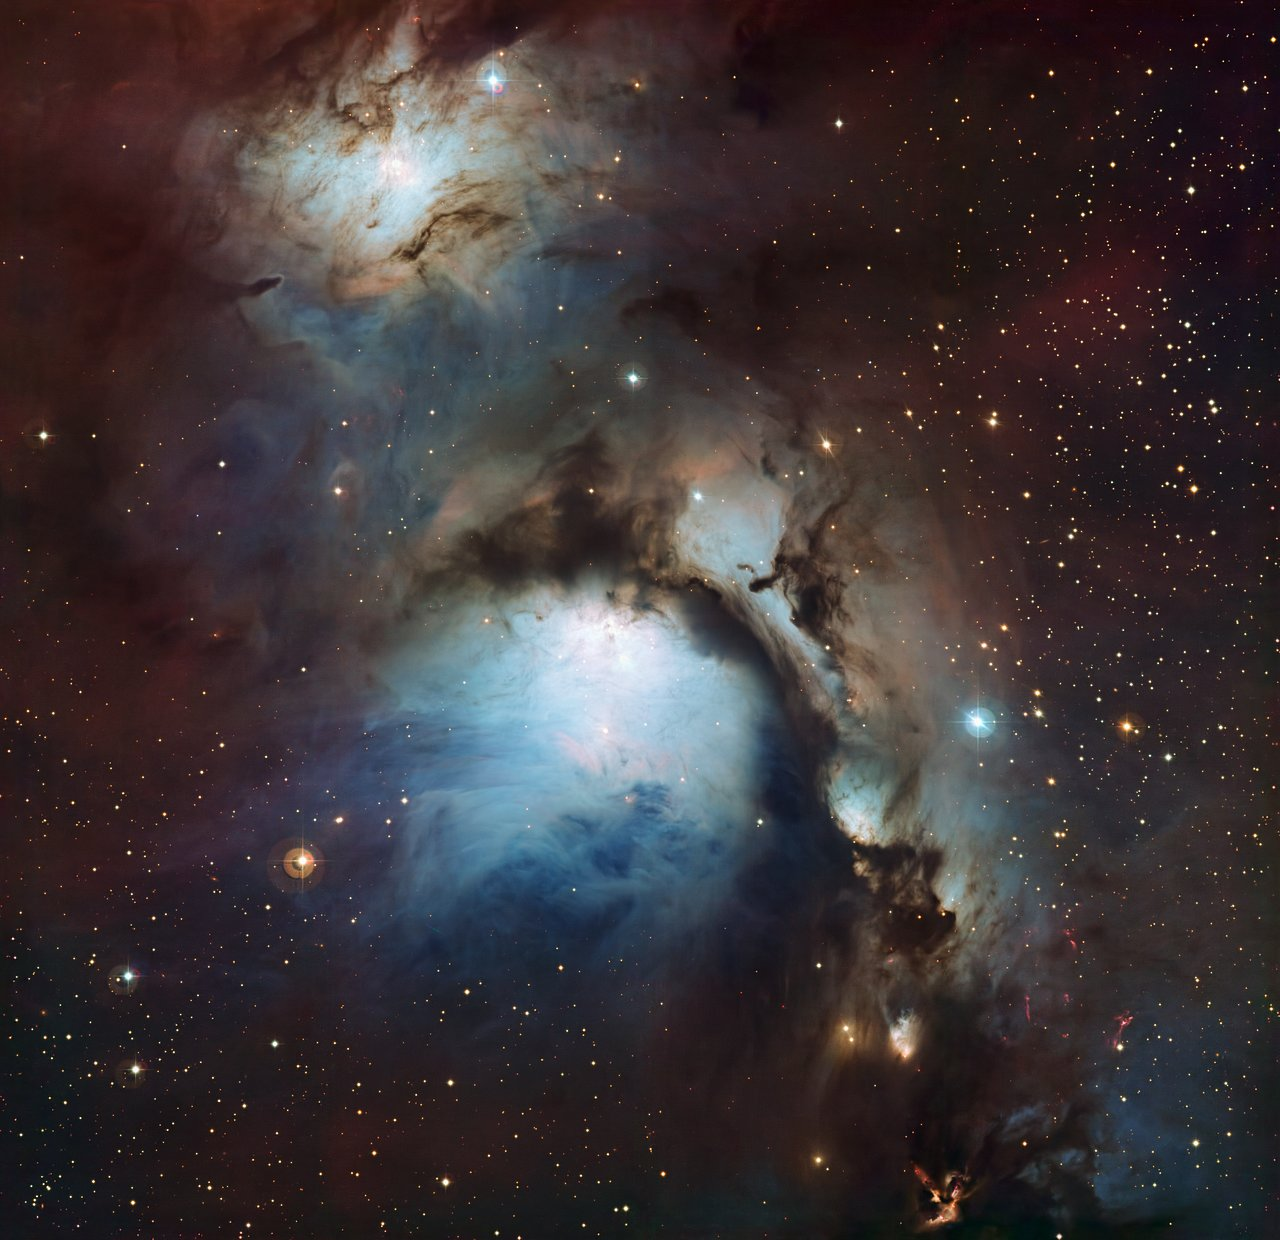
\includegraphics[height=7cm]{img/nebula-messier-78-eso1105a}
		\subcaption{Messier 78 Nebula \footnotemark[1]}
		\label{fig:messier78}
	\end{subfigure}\hfill%
	\begin{subfigure}[c]{0.45\textwidth}
		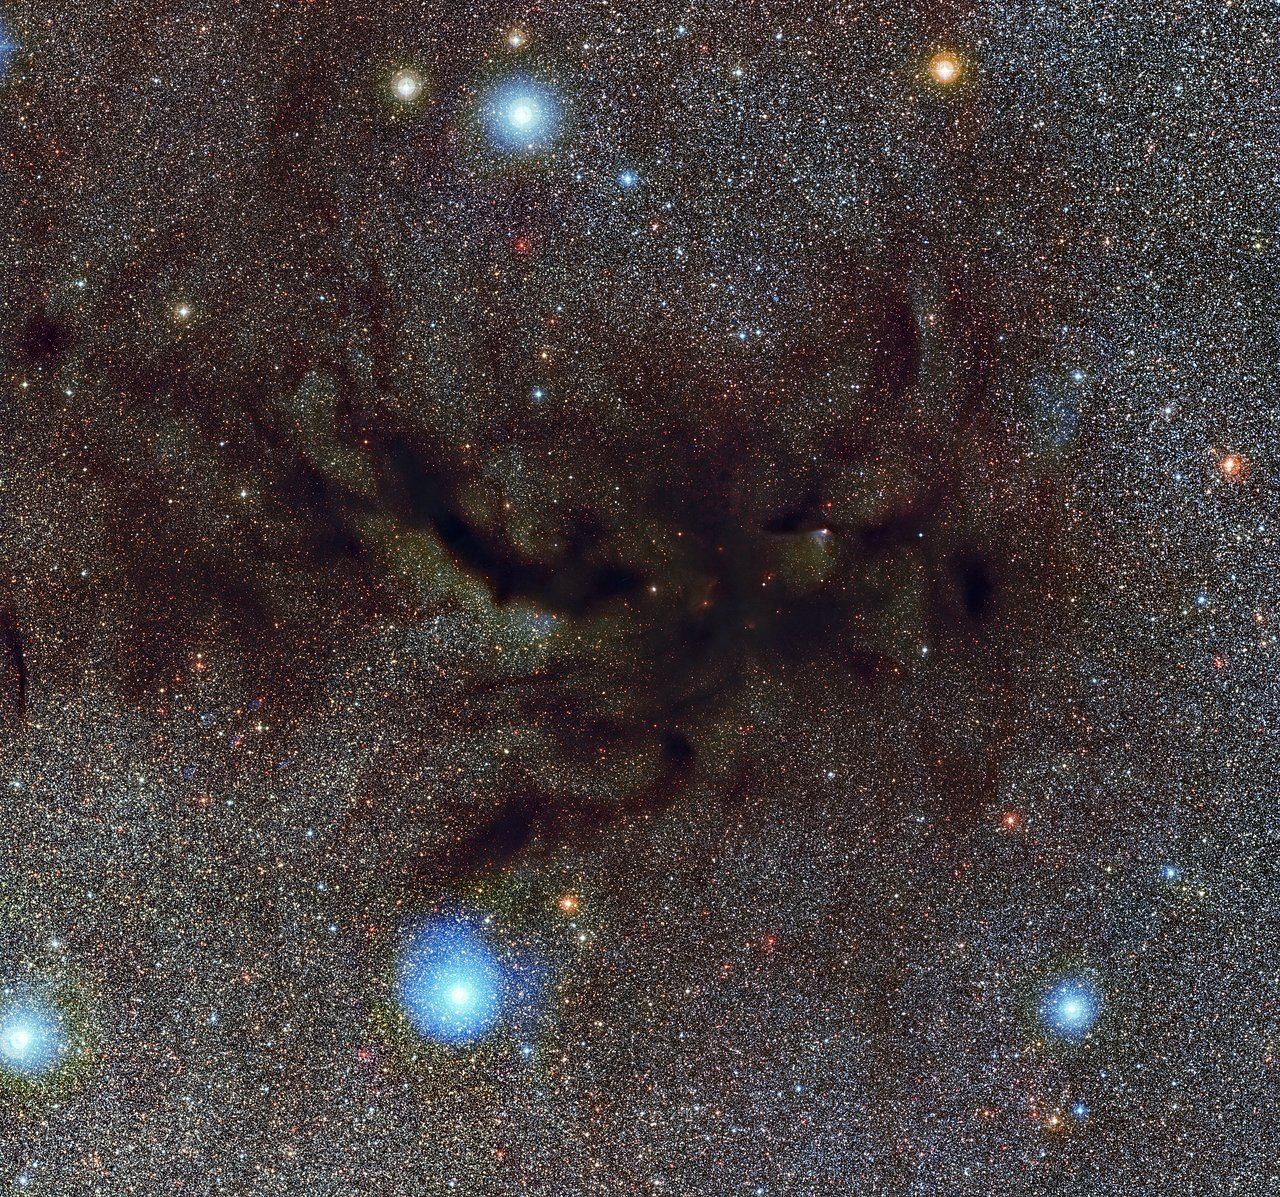
\includegraphics[height=7cm]{img/nebula-pipe-eso1233a}
		\subcaption{Barnard 59, part of the Pipe Nebula \footnotemark[2]}
	\end{subfigure}%
\caption{The dark areas in the figures above are highly dense accumulation of gas, which absorb most of the visibile light from the stars behind them. Inside them are so called "star-nurseries" or star forming regions. The blue regions visibile in \ref{fig:messier78} are caused by reflection of starlight by a high concentration of interstellar dust. The red regions, also visibile in \ref{fig:messier78}, are caused by emission of the heated ISM.}

\label{fig:nebulae}
\end{figure}
\footnotetext[1]{\textbf{Credit:} ESO/Igor Chekalin \url{https://www.eso.org/public/images/eso1105a/}}
\footnotetext[2]{\textbf{Credit:} ESO \url{https://www.eso.org/public/images/eso1233a/}}


An overall, definitive theoretical calculation of star formation is not yet available, given that, apart from complex calculation, the initial conditions are unknown. Qualitatively, it is clear that even the relatively small-scale molecular cloud cores have far too much angular momentum to be able to collapse to stellar dimensions. This problem can be solved by various physical effects, such as:

\begin{enumerate}
\item Fragmentation of the core into a binary or multiple system
\item Collapse of the cloud into a central stellar object surrounded by an orbiting disk,
which contains most of the angular momentum.
\end{enumerate}

\subsection{Star formation phases}

The temperature in the ISM vary grately and in the colder areas ($\rm{\sim 10\, K}$) hydrogen (with some traces of other elements) exists in molecular form in giant molecular clouds. These objects are very inhomogenous, with the densest regions as much as a 1000 times the density of the more rarefied regions (Figure \ref{fig:star-formation:1} \citep{Greene2001}). Inside molecular clouds, the gas pressures are higher than those in the surrounding interstellar medium, and almost all molecular clouds in our galaxy exhibit star formation \citep{Bodenheimer2011}.

\begin{figure}[h]
	\begin{subfigure}[c]{0.3\textwidth}
		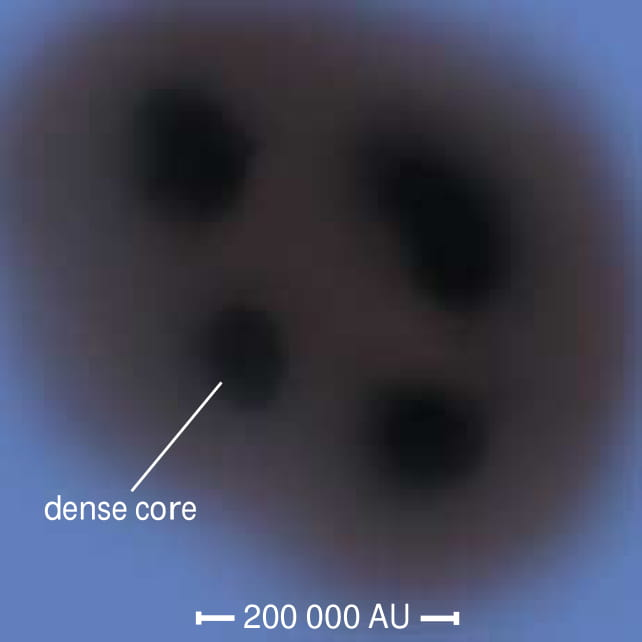
\includegraphics[width=\textwidth]{img/sf1-1}
		\subcaption{Dark cloud}
		\label{fig:star-formation:1}
	\end{subfigure}\hfill%
	\begin{subfigure}[c]{0.3\textwidth}
		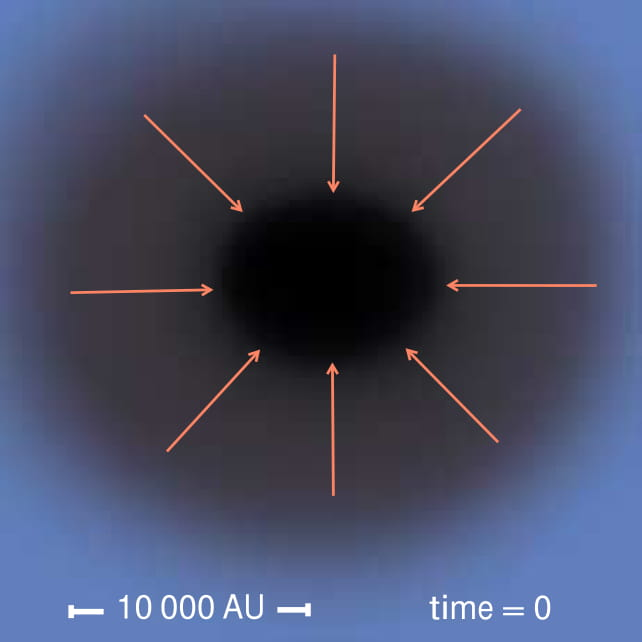
\includegraphics[width=\textwidth]{img/sf2-1}
		\subcaption{Gravitational Collapse}
		\label{fig:star-formation:2}
	\end{subfigure}\hfill%
	\begin{subfigure}[c]{0.3\textwidth}
		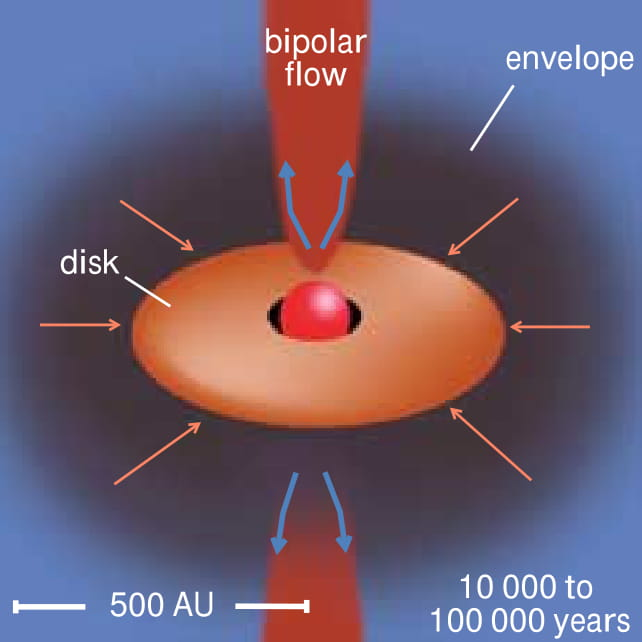
\includegraphics[width=\textwidth]{img/sf3-1}
		\subcaption{Protostar}
		\label{fig:star-formation:3}
	\end{subfigure}%
	\\
		\begin{subfigure}[c]{0.3\textwidth}
		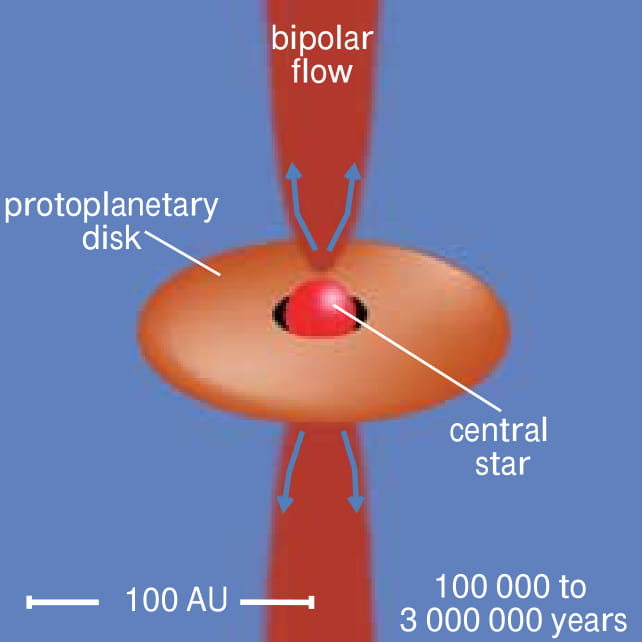
\includegraphics[width=\textwidth]{img/sf4-1}
		\subcaption{Pre-main-sequence-star}
		\label{fig:star-formation:4}
	\end{subfigure}\hfill%
	\begin{subfigure}[c]{0.3\textwidth}
		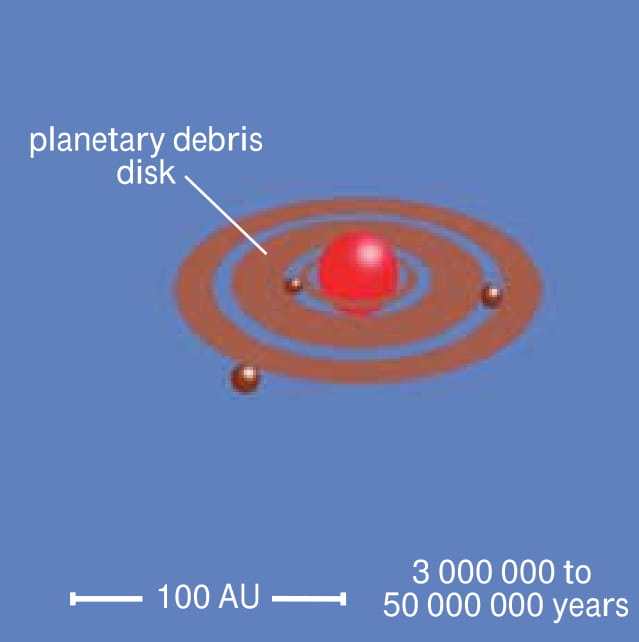
\includegraphics[width=\textwidth]{img/sf5-1}
		\subcaption{T Tauri Star}
		\label{fig:star-formation:5}
	\end{subfigure}\hfill%
	\begin{subfigure}[c]{0.3\textwidth}
		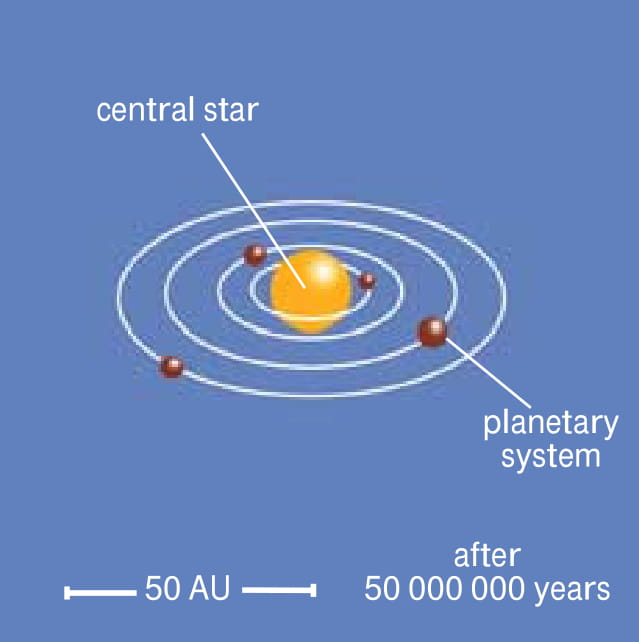
\includegraphics[width=\textwidth]{img/sf6-1}
		\subcaption{Young Planetary system}
		\label{fig:star-formation:6}
	\end{subfigure}%
\caption{The stages of formation of a Sun-like star.}
\label{fig:star-formation}
\end{figure}

Molecular clouds are usually supported against thier weight by thermal pressure, turbulent gas motion and magnetic fields within. By various mechanisms the clouds become unstable and begin to collapse under their own weight (Figure \ref{fig:star-formation:2}). This could be due to long time scale evolution of the cloud or a turbulence, such as supersonic turbulances, random shock interactions in the ISM, supernova shocks, stellar winds and so on \citep{Bodenheimer2011}. At the centre of the collapsing cloud a protostar forms (Figure \ref{fig:star-formation:3}). The protostar continues to  rapidly accumulate mass from the surrounding envelope of gas and dust over the course of about 100 000 years. During its lifetime the protostar progressively increases in density and shrinks in size, accreting the infalling material and sheding mass through bipolar jets. The infalling material, which had been rotating realtively slowly, speeds up as it apporaches the protostar due to conservation of angular momentum. Most matter from the envelope dispres or eventually flows onto the protostar, but some of it falls into orbits of various size depending on its velocity, forming a circumstellar disk. As the accretion process stops, the central globe of gas is no longer considered a protostar: it is now a pre-main-sequence (or PMS) star (Figure \ref{fig:star-formation:4}). Protostars and PMS stars are grouped under the term young stellar objects (or YSO). The pre-main-sequence phase of evolution lasts for tens of millions of years and its earliest phases, these objects are calles T Tauri stars (derived from the archetypical star in the constellation Taurus). With no dusty envelopes, T Tauri stars are the youngest objects that can be observed with an optical telescope. They are surrounded by disk of dust and gas -- often called protoplanetary disk and can continue to eject material in their bipolar jets (Figure \ref{fig:star-formation:5}). After a few million yars, much of the dust and gas in the protoplanetary disk dissipates, leaving a bare PMS star in the centre, sometimes orbited by a few large bodies in a remnant debris disk. In tens of millions of years, the force of gravity eventually triumphs over the outward thermal pressure of the gas within the star and the temperature of the star's interior raises to about 10 million Kelvins -- hot enough to fuse Helium. This marks the arrival of the star on the main-sequence phase of its evolution (Figure \ref{fig:star-formation:6}). This period is extremly stable, and may last for billions of years. The Sun is an example of a main-sequence star, which has been fusing hydrogen into Helium for 5 billions years, and is predicted to do so for 5 billion more. 

\section{Radiation}

Before the properties of pre-main sequence stars and the surronding circumstellar disks can be explored further, it is important to lay down the basics of radiatiative transfer and the underlying radiation mechanisms. 

\subsection{Absorption, emission and scattering}
\label{sec:abs-em-sc}
At atomic level, if the total energy decreases by $\Delta E$ the atom emits a quantum of electromagnetic radiation called a \textit{photon}, whose frequency $\nu$ is determined by the equation \citep{Karttunen2017}:

\begin{equation}
	\Delta E = h \nu,
\end{equation}
where $h=6.6256 \cdot 10^{-34} \rm{Js}$ is the \textit{Planck constant}. Consequently, if the same atom absorbs a photon of frequency $\nu$, it gains energy $\Delta E$.

The energy levels of an electron in an atom are quantized, limitting the frequencies at which an atom can absorb or emit radiation, corresponding to the difference between the initial state $i$ and final state $f$ of the system: $\mid E_{\rm{f}} - E_{\rm{i}} \mid = h\nu_{\rm{fi}}$. A transition from a lower energetic state to a higher energetic state by assimilation of a photon of frequency $h\nu_{\rm{fi}}$ is called \textbf{\textit{excitation}} or \textbf{\textit{absorption}}(Figure \ref{fig:absorption}). A typical lifetime for an excited state is $10^{-8} \, \rm{s}$, after which the atom may return to its lower state, radiating a photon, throught the process of \textbf{\textit{spontaneous emission}} (Figure \ref{fig:spontaneous-emission}). Transitions to lower states (downward) can also be induced by another photon, whose frequency $\nu_{\rm{photon}} = \nu_{\rm{fi}}$ corresponds to the downward transition, interacting and perturbing the excited state. This process called \textbf{\textit{stimulated emission}} (Figure \ref{fig:stimulated-emission}). While spontaneously emitted photons have randomly distributed phases and directions when leaving the atom, producing an incoherent radiation, the radiation produce through stimulated emission is coherent and propagates in the same direction as the induced radiation. \textbf{\textit{Scattering}} is defined as a change in the direction of motion of a particle due to the interaction with the medium (collision with other particle). When refering to electromagnetic radiation, this process can be modeled as absorption of a photon, immediately followed by an instantaneous emission of the photon at the same wavelength, but in a different direction. On the macroscopic scale, the medium seems to reflect the radiation (e.g. atmospheric particles scatter blue light from the Sun). 

\begin{figure}[ht]
	\begin{subfigure}[t]{0.3\textwidth}
		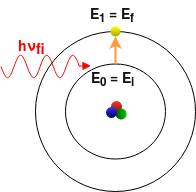
\includegraphics[height=4cm]{img/absorption}
		\subcaption{\textbf{Absorption} occurs when a photon of frequency $\nu_{\rm{fi}}$ is absorbed and the system, initially in a low energy state, is excited to a higher energy state.}
		\label{fig:absorption}
	\end{subfigure}\hfill%
	\begin{subfigure}[t]{0.3\textwidth}
		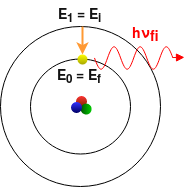
\includegraphics[height=4cm]{img/spontaneous-emission}
		\subcaption{\textbf{Spontaneous emission} is the opposite process to absorption, in the sense that the system emits a photon with the energy corresponding to $\Delta E = h\nu_{\rm{fi}} = h\nu_{\rm{if}}$ as the system goes from the excited state to a lower energy state finally.}
		\label{fig:spontaneous-emission}
	\end{subfigure}\hfill%
	\begin{subfigure}[t]{0.3\textwidth}
		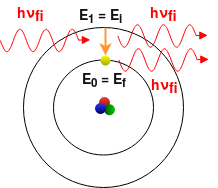
\includegraphics[height=4cm]{img/stimulated-emission}
		\subcaption{\textbf{Stimulated emission} is the process in which emission occurs after a photon with exactly the same frequency as the emitted photon $h\nu_{\rm{fi}}$ interacts with the excited state.}
		\label{fig:stimulated-emission}
	\end{subfigure}\hfill%
	\begin{subfigure}[c]{1.0\textwidth}
		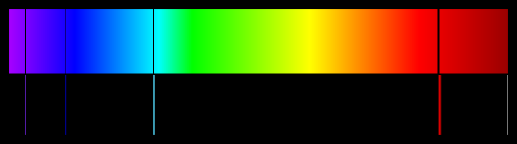
\includegraphics[width=\textwidth]{img/hydrogen-spectra}
		\subcaption{Hydrogen Spectra: absorption (top) lines can be seen as dark (missing) lines against the continuous spectra of light \& emission (bottom) lines in color ar at the same frequency as the corresponding absorption between the same states.}
		\label{fig:hydrogen-spectra}
	\end{subfigure}
\caption{Spectral lines origin}
\label{fig:spectra}
\end{figure}%

Through absorption, spontaneous emission and stimulated emission the system's energetic states can change (Figure \ref{fig:spectra}), this gives rise to an element-specific line spectrum (see \ref{fig:hydrogen-spectra} for Hydrogen). A hot gas under low pressures produces an emission spectrum of discrete lines. The same gas at a cooler temperature observed against a source of white light (continuous spectrum) shows dark absorption lines at the corresponding frequencies for the same transitions as the emission lines\citep{Karttunen2017}. In reality, the specral lines are not infinetly narrow and sharp, but are somewhat broadened, having a shape called a line profile. There are various factors which contribute to line broadening, an intrisic one being \textit{Heisenberg's uncertainty principle} ($\Delta E \Delta t \approx \hbar$). AS a consequence, if a state has a lifetime $\tau_k$, its corresponding energy can only physically be determied with an accuracy of $\Delta E_k = \hbar/\tau_k$. The uncertainty in the energy levels (And therefore in the wavelength) involved in a transition depends on the lifetimes of both the final and initial states, giving a \textbf{\textit{natural line width}} $\gamma$ (\ref{eq:nlw}). If only this effect is taken into consideration, the width $\gamma$ is equal to the full width at half maximum (FWHM), as this is the width of the line profile at a depth where the intensity is half of the maximum. 

\begin{equation}\label{eq:nlw}
	\gamma = \frac{1}{\tau_{\rm{i}}} + \frac{1}{\tau_{\rm{f}}}
\end{equation}

The higher the temperature of a gas, the faster atoms move, causing the spectral lines to move due to the \textit{Doppler effect}, thus, the shape of the line depends on the velocity distribution of individual atoms. The line profile due to Doppler shifts is calles a Voing profile, and is less sharp than the natural line profile, having a greater full width at half maximum. Other effects include pressure broadening and non-local broadening. 

\subsection{Blackbody radiation}

A \textbf{\textit{blackbody}} is a physically ideal object, which does not reflect or scatter radiation, but absorbs and re-emits radiation completely. Black holes are near-perfect black bodies, as they absorb all the incident radiation, and although planets and stars are not perfect blackbodies, black-body radiation is a good first approximation for the thermal energy they emit. The wavelength distribution of the radiation follows \textit{Planck's Law} and depends only on the temperature $T$ of the blackbody. The intensity $B$ of the radiation at frequency $\nu$ is given by:
\begin{equation}\label{eq:planck}
	B_\nu(T) 
	=\frac{2h\nu^3}{c^2}\frac{1}{e^{h\nu/kT}-1},
\end{equation}	 
where $h$ is \textit{Planck's constant}, $c$ is the \textit{speed of light} ($3 \cdot 10^8 \, \rm{ms^{-1}}$), and $k$ is the \textit{Boltzmann constant} ($1.38 \cdot 10^{-23} \, \rm{JK^{-1}}$), giving the intensity $B_\nu$ the dimension $\rm{W m^{-2} Hz^{-1} sterad^{-1}}$. The distribution can also be written as a function of wavelength: 

\begin{equation}
	B_\lambda(T) 
	=\frac{2hc^2}{\lambda^5}\frac{1}{e^{hc/\lambda kT}-1},
\end{equation}	

\begin{figure}[h]
		\centering
		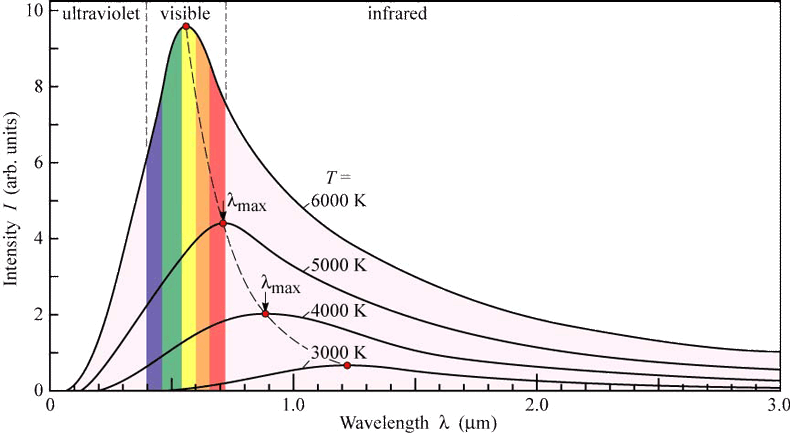
\includegraphics[width=0.8\textwidth]{img/planck-distribution}
		\caption{Intensity distribution of black bodies at different temperatures according to Planck's Law. The Sun, with a temperature of $5780 \rm{K}$ peaks in the area fo the spectrum corresponding to visible light. \citep{Openstax:Physics}}
		\label{fig:planck-distrib}
\end{figure}
 
The total intensity can be calculated by integrating over the spectrum:
\begin{equation}\label{eq:intensity}
	B(T) 
	=\int_{0}^{\infty} B_\lambda(T) \diff \lambda
	=\int_{0}^{\infty} B_\nu(T) \diff \nu 
\end{equation}

By replacing (\ref{eq:planck}) into (\ref{eq:intensity}) and taking out the independet variables the following is obtained:

\begin{equation}\label{eq:integral}
	B(T) 
	=\frac{2h}{c^2} \int_{0}^{\infty} \frac{\nu^3}{e^{h\nu/kT}-1} \diff \nu 
\end{equation}

Integrating by substitution of the integration variable with $x = h\nu/(kT)$, $\diff \nu =kT \diff x/h$  in (\ref{eq:integral}) the following is obtained:

\begin{equation}\label{eq:integral2}
	B(T) 
	=\frac{2h}{c^2}\frac{k^4}{h^4} T^4 \int_{0}^{\infty} \frac{x^3}{e^{x}-1} \diff x
	=\frac{2k^4}{c^2h^3}\frac{\pi^4}{15} \, T^4 
\end{equation}

The integral in (\ref{eq:integral2}) is not easy to evaluate, but it can easily be seen that it is constant in value (independent of temperature). The flux density $F$ for isotropic radiation of intensity $B$ is $F=\pi B$ so the flux can be written as:

\begin{equation}\label{eq:sfl}
	F
	=\sigma T^4. 
\end{equation}

Equation (\ref{eq:sfl}) is the \textit{Stefan-Boltzmann Law}, with $\sigma = 5.67 \cdot 10^{-8}\rm{W m^{-2} K^{-4}}$, the \textit{Stefan-Boltzmann constant}. 

\subsection{Radiative Transfer} %TODO move Circustellar disk section? %

The mechanism through which energy is transfered through the propagation of radiation through a medium is called radiative transfer. The propagation of radiation through a medium is gouverened by the aforementioned phenomena of absorption, emission, and scattering, where absorption leads to a gain in energy, emission leads to a loss of energy and scattering represents the redistribution of energy. The equation of radiative transfer can be easily derived. 

Assume a source, such as a star, which is radiating like a blackbody at temperature $T$, and a small area of space, in a form of a cylinder of area $dA$, and radius $dr$, at a distance $d$ from the source, such that it spans the solid angle $d\omega$: Figure \ref{fig:rad-trans}.

\begin{figure}[h]
	\centering
	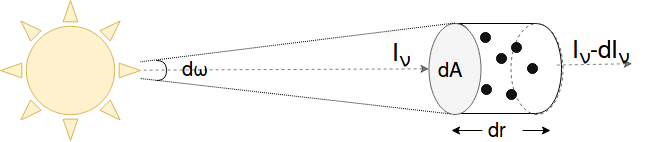
\includegraphics[width=\textwidth]{img/rad-trans}%
  	\caption{}
  	\label{fig:rad-trans}
\end{figure}

If the intensity changes by an amount $dI_{\nu}$ going thorugh the cylinder, than in the time interval $dt$, the energy changes by:
%
\begin{equation}\label{eq:energy-total}
	dE = dI_\nu dA d\nu d\omega dt
\end{equation}
%
This energy difference must be equal to the absorption minus the emission in the cylinder element. The fraction of absorbed energy depends on the opacity of the medium at the given frequency $\nu$:
%
\begin{equation}\label{eq:energy-absorption}
	dE_{\rm{abs}} = \alpha_{\nu} I_{\nu} dr dA d\nu d\omega dt
\end{equation}
%
Let the emission coefficient of the medium be $j_{\nu}$, describing the amount of energy emitted at frequency $\nu$, per Hertz, per unit time, into unit solid angle from unit volume, then the energy emitted is:
%
\begin{equation}\label{eq:energy-emission}
	dE_{\rm{em}} = j_{\nu} dr dA d\nu d\omega dt
\end{equation}
%
By replacing (\ref{eq:energy-total}), (\ref{eq:energy-absorption}), (\ref{eq:energy-emission}) into the equation for conservation of energy 
%
\begin{equation}
	dE = -dE_{\rm{abs}} + dE_{\rm{em}},
\end{equation}
%
one obtains:
%
\begin{equation}
	dI_{\nu}= - \alpha_{\nu} I_{\nu} dr  + j_{\nu} dr
\end{equation}
%
or
%
\begin{equation}\label{eq:rad-transf-1}
	\frac{dI_{\nu}}{\alpha_{\nu}dr} = -I_{\nu} + \frac{j_{\nu}}{\alpha_{\nu}}
\end{equation}

The \textbf{\textit{optical depth}}, $\tau$, in astrophysics is a measure of the extinction coefficient or absorptivity of a medium at a certain frequency $\nu$. Therefore the total optical depth, expressing how much of the light will be absorbed by the medium through a certain path is the integral sum of the extinction coefficient 	$\alpha_{\nu}$ along that path: 
\begin{equation}\label{eq:optical-depth}
	\tau_{\nu} = \int_0^r \alpha_{\nu} dr = \sigma N
\end{equation},
%
and it can also be expressed in terms of the number density $N$ and the cross section $\sigma$. From the definition one can understand that an optically thick material, with a high value for the optical depth $\tau$, is highly obscuring and does not let much of the light pass through. Figure \ref{fig:barnard68} exemplifies this with a real celestial object. 

The \textit{source function} $S_\nu$ is a measure of the emission to absorbtion coefficient in the case of no scattering, indicateing how many photons are removed and replaced by new ones as a beam of light passes through the material:

\begin{figure}[ht]
	\begin{subfigure}[t]{0.47\textwidth}
		\includegraphics[height=7.5cm]{img/barnard-68-eso0102a2}
		\subcaption{Barnard 68 three-color composite reproduced from one blue (B), one green-yellow (V) and one near-infrared (I) exposure \footnotemark[1]}
		\label{fig:barnard68-vis}
	\end{subfigure}\hfill%
	\begin{subfigure}[t]{0.47\textwidth}
		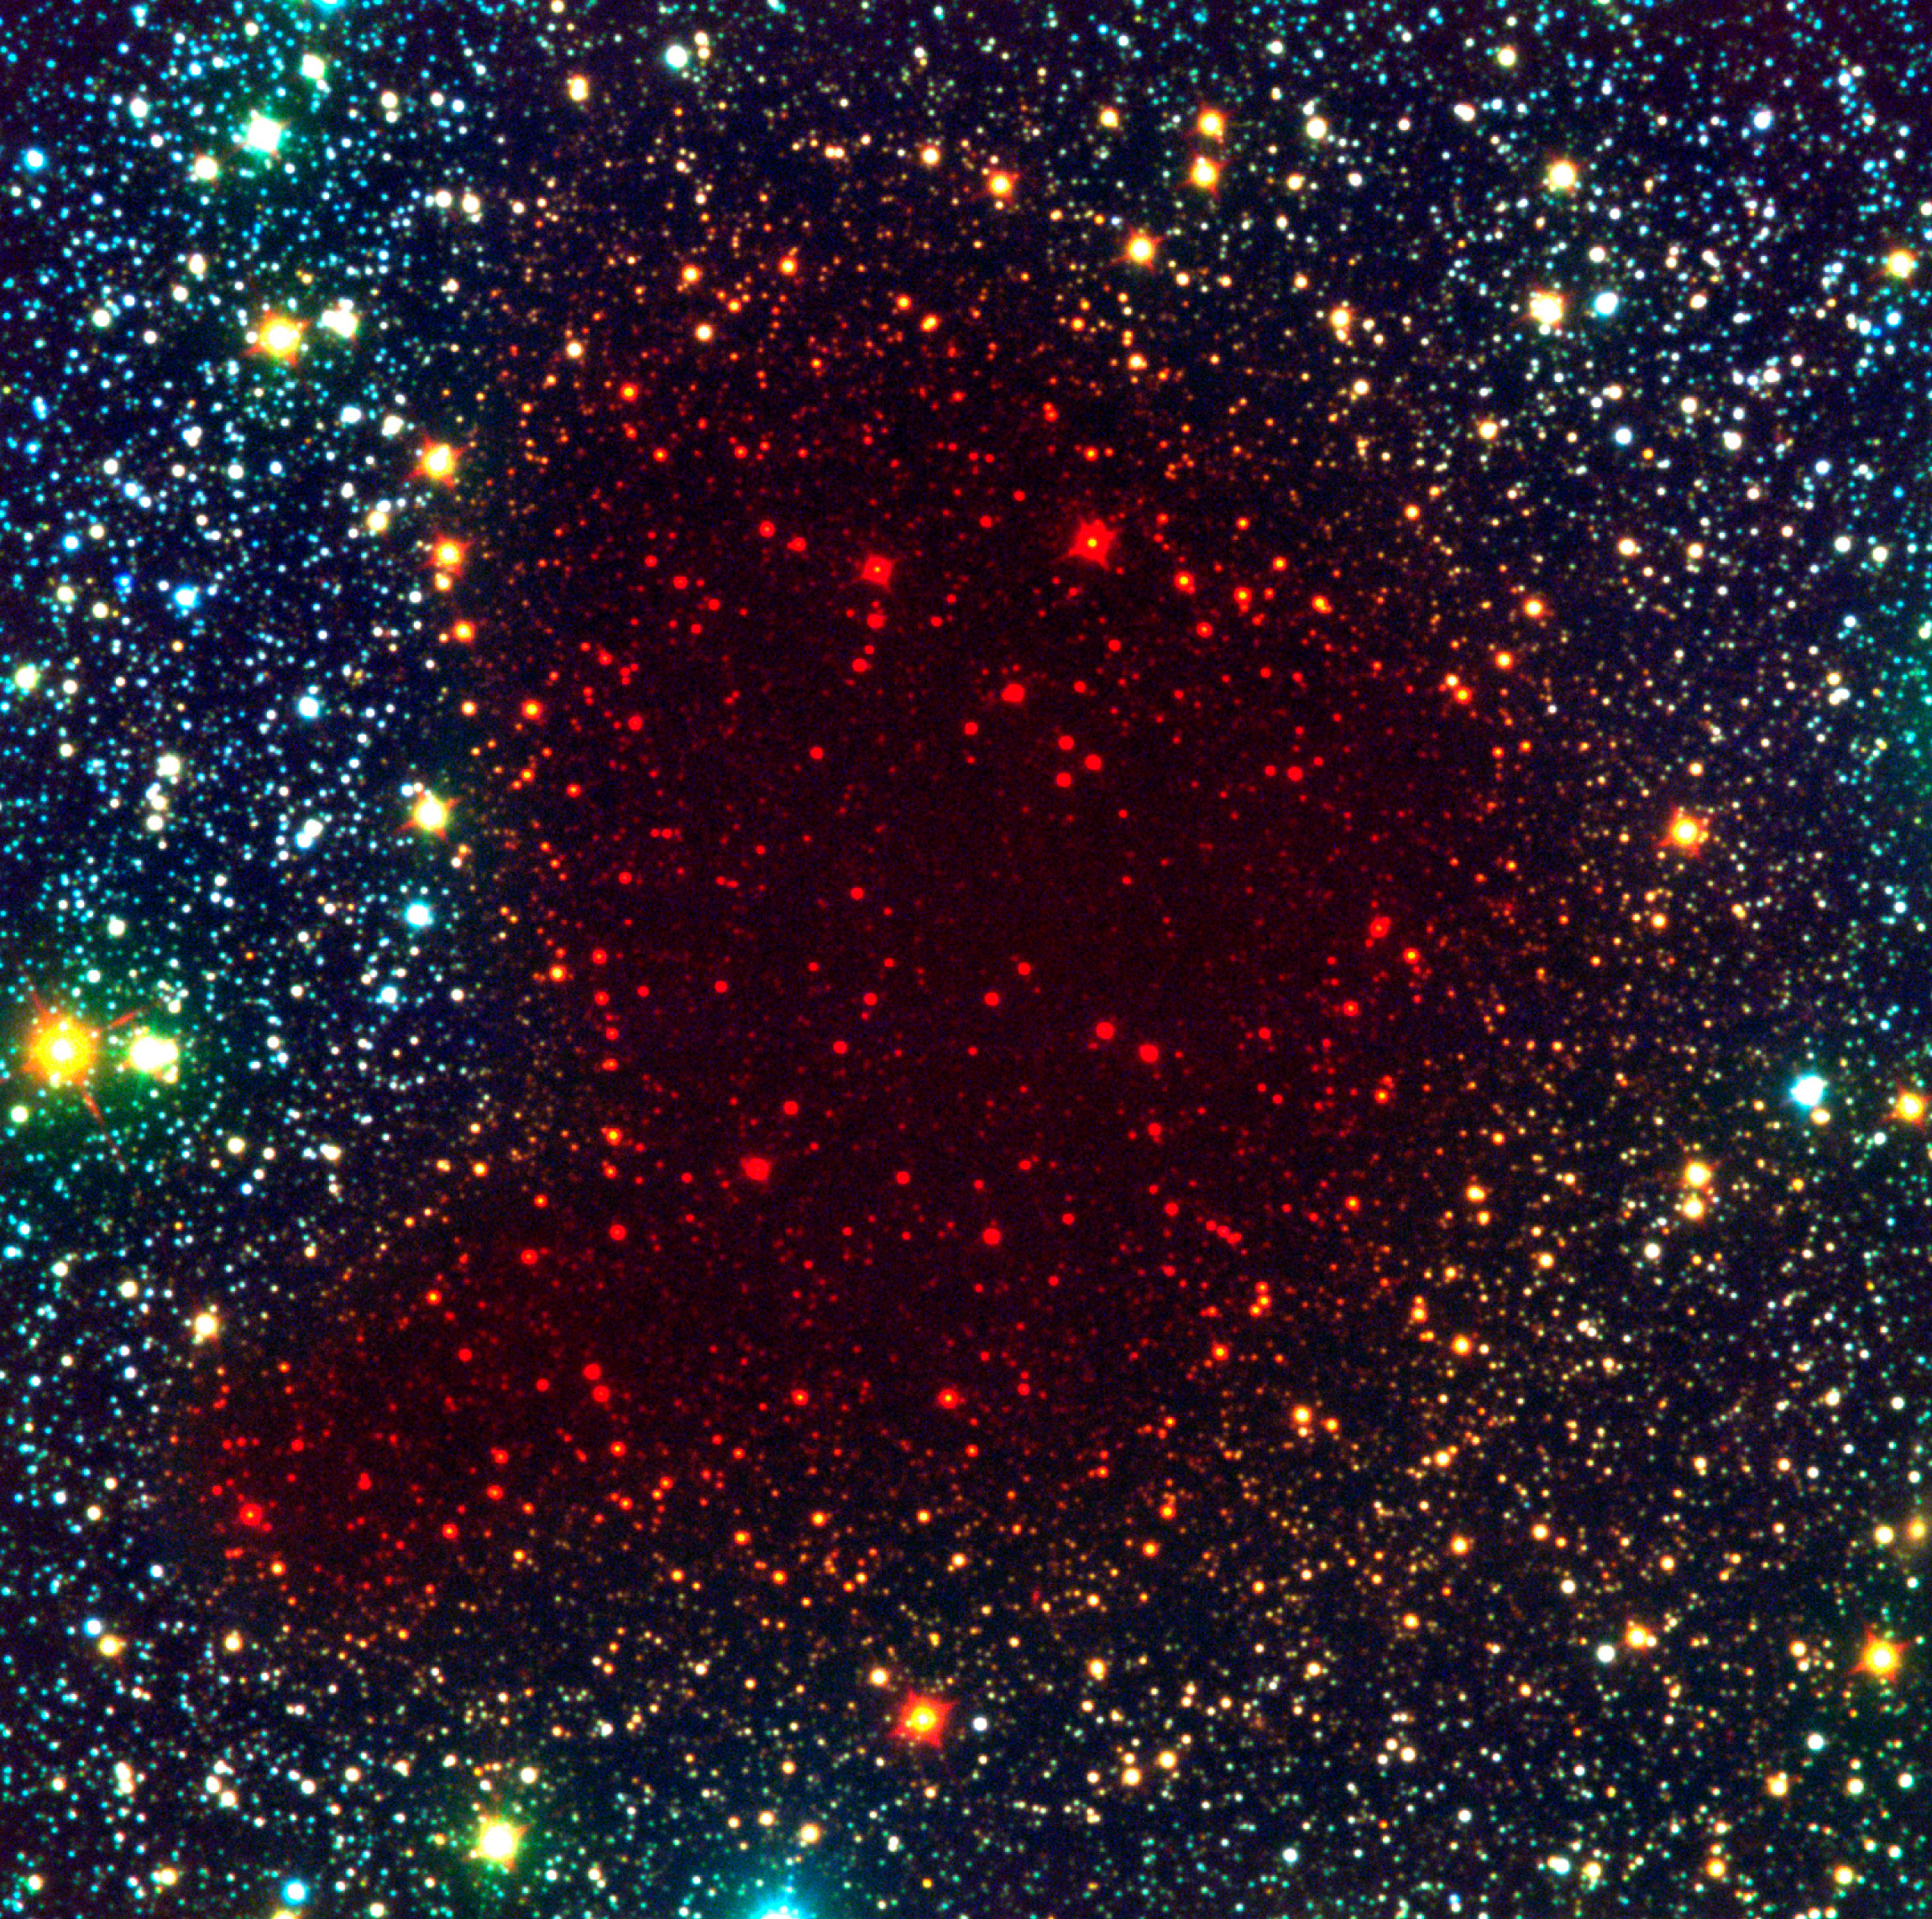
\includegraphics[height=7.5cm]{img/barnard-68-ir-eso0102b}
		\subcaption{Barnard 68, false-colour composite based on a visible (here rendered as blue), a near-infrared (green) and an infrared (red) image \footnotemark[2]}
		\label{fig:barnard68-ir}
	\end{subfigure}%
\caption{Comparing the two composite expostions of the same astronomical object, it can be clearly seen in \ref{fig:barnard68-vis} that the globule is optically thick for the visible spectrum, not letting any light from the stars behind pass through, while in \ref{fig:barnard68-ir} a multitude of stars appear in the infrared, colored red in the image, making the globule opthically thin in the infrared region of the spectrum.}
\label{fig:barnard68}
\end{figure}
\footnotetext[1]{\textbf{Credit}: ESO, \url{https://www.eso.org/public/images/eso0102a/}}
\footnotetext[2]{\textbf{Credit}: ESO, \url{https://www.eso.org/public/images/eso0102b/}}

\begin{equation}\label{eq:source-function}
	S_{\nu} = \frac{j_{\nu}}{\alpha_{\nu}}
\end{equation}

By replacing the newly defined optical depth (\ref{eq:optical-depth}) and source function (\ref{eq:source-function}) into the derived equation (\ref{eq:rad-transf-1}) from the conservation of energy, the following is obtianed:

\begin{equation}\label{eq:rad-transf}
	\frac{dI_{}\nu}{d\tau_{\nu}} = -I_{\nu} + S_{\nu}
\end{equation}

Equation (\ref{eq:rad-transf}) is the basic equation of radiative transfer. If the incident intensity $I_{\nu} < S_{\nu}$ is smaller than the source function, the intensity increseas in the direction of propagation, meaning also the medium is emitting more than it is absorbing for the given freqeuncy $\nu$. Whereas, if the incident intensiy is larges than the source function $I_{\nu} > S_{\nu}$, then $dI_{\nu}/d\tau < 0$ and the outgoing intensity will be smaller, meaning the medium is oabsorbant or optically thick at the given frequency. In equilibrium, the emitted and absorbed energies are equal, $I_{\nu} = S_{\nu}$, and the radiation of the medium is that of a blackbody, with the source function given by:

\begin{equation}
	S_{\nu} = B_{\nu}(T) = \frac{2h\nu^3}{c^2} \frac{1}{\exp{h\nu/kT}-1}
\end{equation}

A formal solution to the radiative transfer equation (\ref{eq:rad-transf}) for the outgoing intensity is made up of an exponentially decay of the initial intensity (denoted $I_{\nu}(0)$) with the absorption coefficient plus the emission of the medium at the given frequency:

\begin{equation}\label{eq:solution}
	I_{\nu}(\tau_{\nu}) = I_{\nu}(0)\exp{-\tau_{\nu}} + \int_0^{\tau_{\nu}} \exp{-(\tau_{\nu}-t)} S_{\nu}(t) dt
\end{equation}

The solution is only formal as $S_{\nu}$ is usually unkown must be solved for simultaneously with the intensity.

\section{Stellar properties}

\subsection{Effective Temperature $T_e [\rm{K}]$}

Temperatures in the Universe range from $\rm{0 K}$ to millions of degrees, and the measure of the temperature depends on the physical phenomena underlying the definition of temperature. The most useful way to obtain a temperature is by fitting it against a blackbody spectra. The \textbf{\textit{effective temperature $T_e$}} refers to the surface of the star and is defined as the temperature of a blackbody which radiates with the same total flux density as the star. In other words, for a value of the $T_e$ which ensures the Stefan-Boltzmann law gives the correct flux density $F$ on the surface of the star, we have found the effective temperature. From (\ref{eq:sfl}), the flux density at the surface  becomes then

\begin{equation}\label{eq:sfl}
	F
	=\sigma T_e^4. 
\end{equation}

\subsection{Luminosity $L_\star [\rm{L_\odot}]$}

The luminosity of a star is given by the total energy radiated per second from its surface. It can be callculated for a specific wavelength, or for all wavelengths (\textbf{Bolometric luminosity}). The brightness of the star as measured from Earth is called \textbf{Apparent Magnitude}\footnote[1]{The \textbf{Absolute Magnitude} of a star is defined as the apparent magnitude at exactly $10\, \rm{parsec}$ from the star.} and it does not accurately describe the star's luminosity, as it is also dependent on the distance from the Earth to the star. Given that at a distance $r$ form the source (star), the same amount of energy is spread to a sphere of surface are $4\pi r^2$, the flux density F falls off proportionally to $1/r^2$, as represented in Figure \ref{fig:inverse-square-law}. Assuming an isotropically radiating star of luminosity $L$, the flux $F$ at a distance $r$ from the star would be given by the relation \cite{Karttunen2017}:

\begin{equation}\label{eq:lum}
	L = 4\pi r^2 F
\end{equation}

By replacing $F$ from (\ref{eq:sfl}) in equation (\ref{eq:lum}) we obtain the relationship between the radius, temperature and luminosity of a star. 

\begin{equation}\label{eq:essential-relation}
	L = 4\pi\sigma R^2 T_e^4 
\end{equation}

\begin{figure}[h]
	\centering
	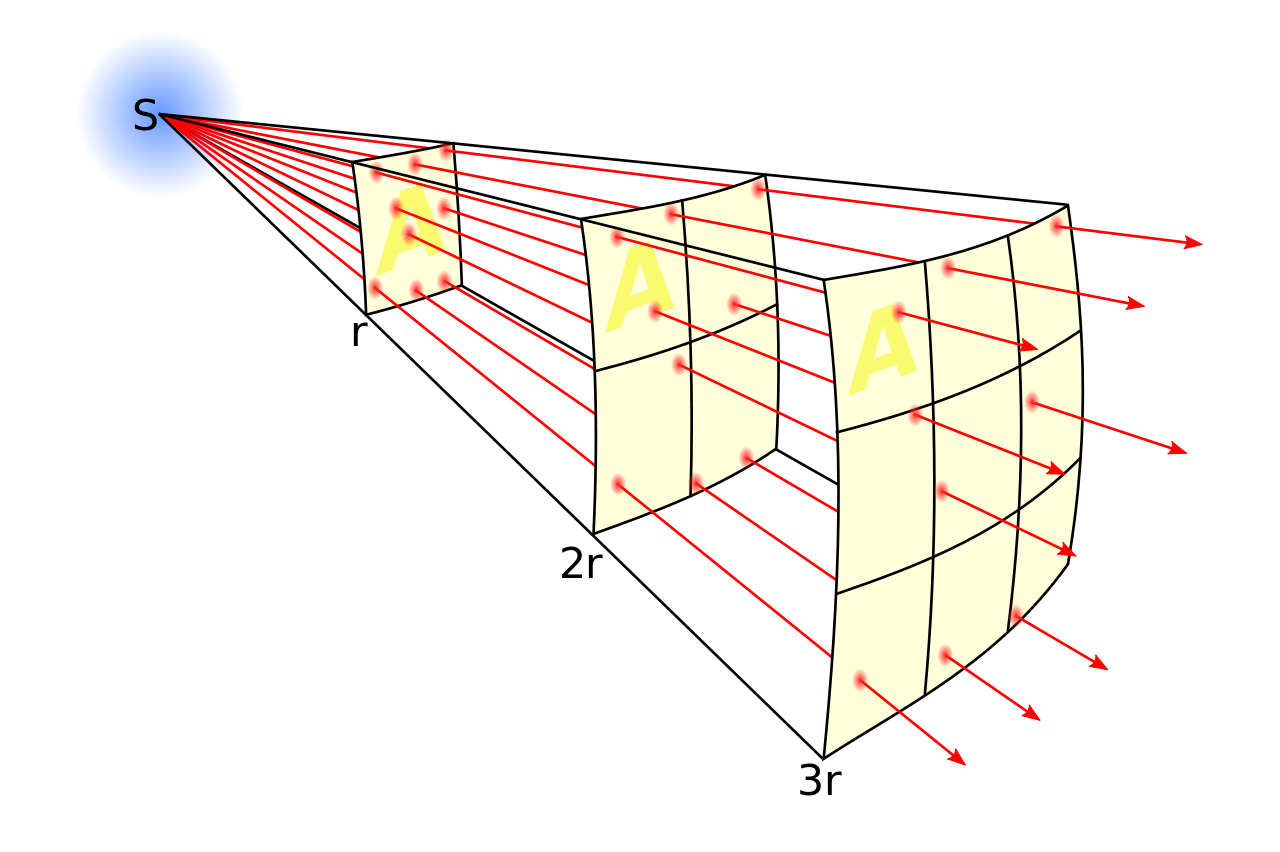
\includegraphics[width=0.6\textwidth]{img/inverse-square-law}%
  	\caption{Inverse square law \protect\footnotemark[1]: As the radius increases from $r$ to $2r$, the same radiation passes now through 4 times the surface area $A$, and as the radius increase to $3r$, the surface area increases to $9A$.}
  	\label{fig:inverse-square-law}
\end{figure}
\protect\footnotetext[2]{By Borb, CC BY-SA 3.0, \url{https://commons.wikimedia.org/w/index.php?curid=3816716}}

\subsection{Stellar Mass $M_\star[\rm{M_\odot}]$}
Stars are massive gaseos bodies which generate energy through nuclear fusion in the core, and release it as radiation. The mass of the star $M_\star$ (usually expressed in terms of the mass of the Sun $\rm{M_\odot}$ determines the star's properties (such as temperature, luminosity and size), but most importantly its evolution track. The pressure of the energy emitted from the core would cause the star to explode, were it not counteracted by the gravity of the surrounding material. When the sum of the gravitational and pressure force acting on a volume element is zero (Figure \ref{fig:hydrostatic-equilibrium}), hydrostatic equilibrium is reached, and the star is stable. 

\begin{figure}[h]
		\centering
		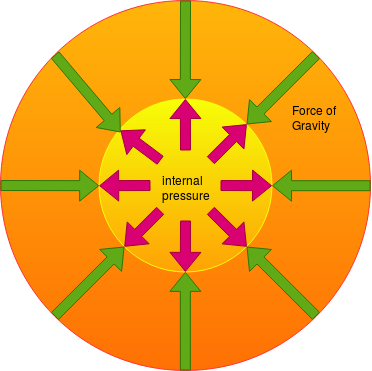
\includegraphics[width=0.37\textwidth]{img/hydrostatic-equilibrium}%
  		\caption{ Hydrostatic equilibrium in stellar interiors is achieved when the \textbf{\textcolor{FrogGreen}{gravitational force}} matches the \textbf{\textcolor{Fuchsia}{internal pressure}} at each point.}
  		\label{fig:hydrostatic-equilibrium}
\end{figure}

When the balance changes, however, so does the state of the star. Stars can have masses in a relatively small interval: if the mass of a star is less than $\rm{0.08\,  M_\odot}$ or bigger than $\rm{100\,  M_\odot}$ the star becomes unstable \citep{Reese2005}. The smallest stellar masses observed are about about $0.05 \rm{M_\odot}$, and the largest one could be up to $150 \rm{M_\odot}$ \citep{Karttunen2017}. These values are however approximate as they are based on an empirical mass–luminosity relation, which can be used to estimate stellar masses: 

\begin{equation}
	L \propto M^{3.8}
\end{equation}

It is important to note that the relations is only approximate, and can be considered valid for main-sequence stars. The only stars with accurately known masses are the ones found in binary systems, where the masses of the individual components
can be determined by observing the motions of both components relative to the centre of mass. Less than half of all stars are single stars like the Sun, while more than 50 \% belong to system consisting of two or more members (which is binary at some level). 


\subsection{Spectra}

Most of the important information about the physical properties of stars come from studies of their spectra \citep{Karttunen2017}. By means of dispresing the incoming light from stars we can observe their spectra and compare it to the spectra of known elements (e.g. the spectra of Hydrogen in Figure \ref{fig:hydrogen-spectra}, see appendix A). 

The spectral classification scheme used at present is called the Harvard classification, as it was developed at the Harvard Observatory at the beginning of the 20\textsuperscript{th} century by Annie Jump Cannon, and published in the Henry Draper Catalogue. The classification is based on lines that are mainly sensitive to the stellar temperature, such as the hydrogen Balmer lines, the lines of neutral helium, the iron lines and others mentioned in Table \ref{table:spectra}.

The spectral types were denoted alphabetically with a capital letter, subsequently, in order of decreasing temperature the classification became 
\begin{center}
C\\
O–B–A–F–G–K–M–L–T\\
S\\
\end{center}
with some additional notations (Q for novae, P for planetary nebulae and W for Wolf–Rayet stars). The spectral classes C and S represent parallel branches to types G–M, differing in their surface chemical composition. The most recent addition
are the spectral classes L and T continuing the sequence beyond M, representing brown dwarfs. The spectral classes are divided into subclasses denoted by the numbers $\overline{0..9}$, with decimal sometimes being used.

\begin{table}[h!]
	\begin{center}
 		\begin{tabular}{|c | l | l r| l|} 
		\hline
 		Type & Proeminent Spectral Lines & Color & & Temperature \\ [0.5ex] 
 		\hline
 		O & He\textsuperscript{+}, He, H, O\textsuperscript{2+}, N\textsuperscript{2+}, C\textsuperscript{2+}, Si\textsuperscript{2+} & Blue & \tikz\draw[fill=OBlue] (0,0) circle (1ex);  & $\sim$ 30 000 K \\ 
 		\hline
 		B & He, H, C\textsuperscript{+}, O\textsuperscript{+}, N\textsuperscript{+}, Fe\textsuperscript{2+}, Mg\textsuperscript{2+} & Blue-white & \tikz\draw[fill=BBlue] (0,0) circle (1ex);  & 15 000 K \\ 
 		\hline
 		A & He, ionized metals & White & \tikz\draw[fill=white] (0,0) circle (1ex);  & 9 000 K \\ 
 		\hline
 		F & H, Ca\textsuperscript{+}, Ti\textsuperscript{+}, Fe\textsuperscript{+} & Yellow-white & \tikz\draw[fill=FYellow] (0,0) circle (1ex);  & 7 000 K \\
  		\hline
 		G & Ca\textsuperscript{+}, Fe, Ti, Mg, H, some molecular bands & Yellow & \tikz\draw[fill=yellow] (0,0) circle (1ex);  & 5 500 K \\
 		\hline
 		K & Ca\textsuperscript{+}, H, molecular bands & Orange & \tikz\draw[fill=orange] (0,0) circle (1ex);  & 4 000 K \\
 		\hline
 		M & TiO, Ca, molecular bands & Red & \tikz\draw[fill=red] (0,0) circle (1ex);  & $\sim$  3 000 K  \\ [1ex] 
 		\hline
		\end{tabular}
	\caption{Spectral stellar types}
	\label{table:spectra}
	\end{center}
\end{table}

An alternative to the Harvard classification, which only takes into accout the effect of temperature on the spectrum, is the Yerkes or MKK classification, which takes into account the luminosity of the stars (even for the same effective temperature), determined from spectral lines that depend strongly on the stellar surface gravity, which is closely related to the luminosity. 
Six different luminosity classes are distinguished, denoted by Roman numerals (the Sun is G2 V):

\begin{itemize}[noitemsep]
\item Ia most luminous supergiants
\item Ib less luminous supergiants
\item II luminous giants
\item III normal giants
\item IV subgiants
\item V main sequence stars (dwarfs)
\end{itemize}

\subsection{HR Diagram}

% HR DIAGRAM
\begin{figure}[hbt!]
		\centering
		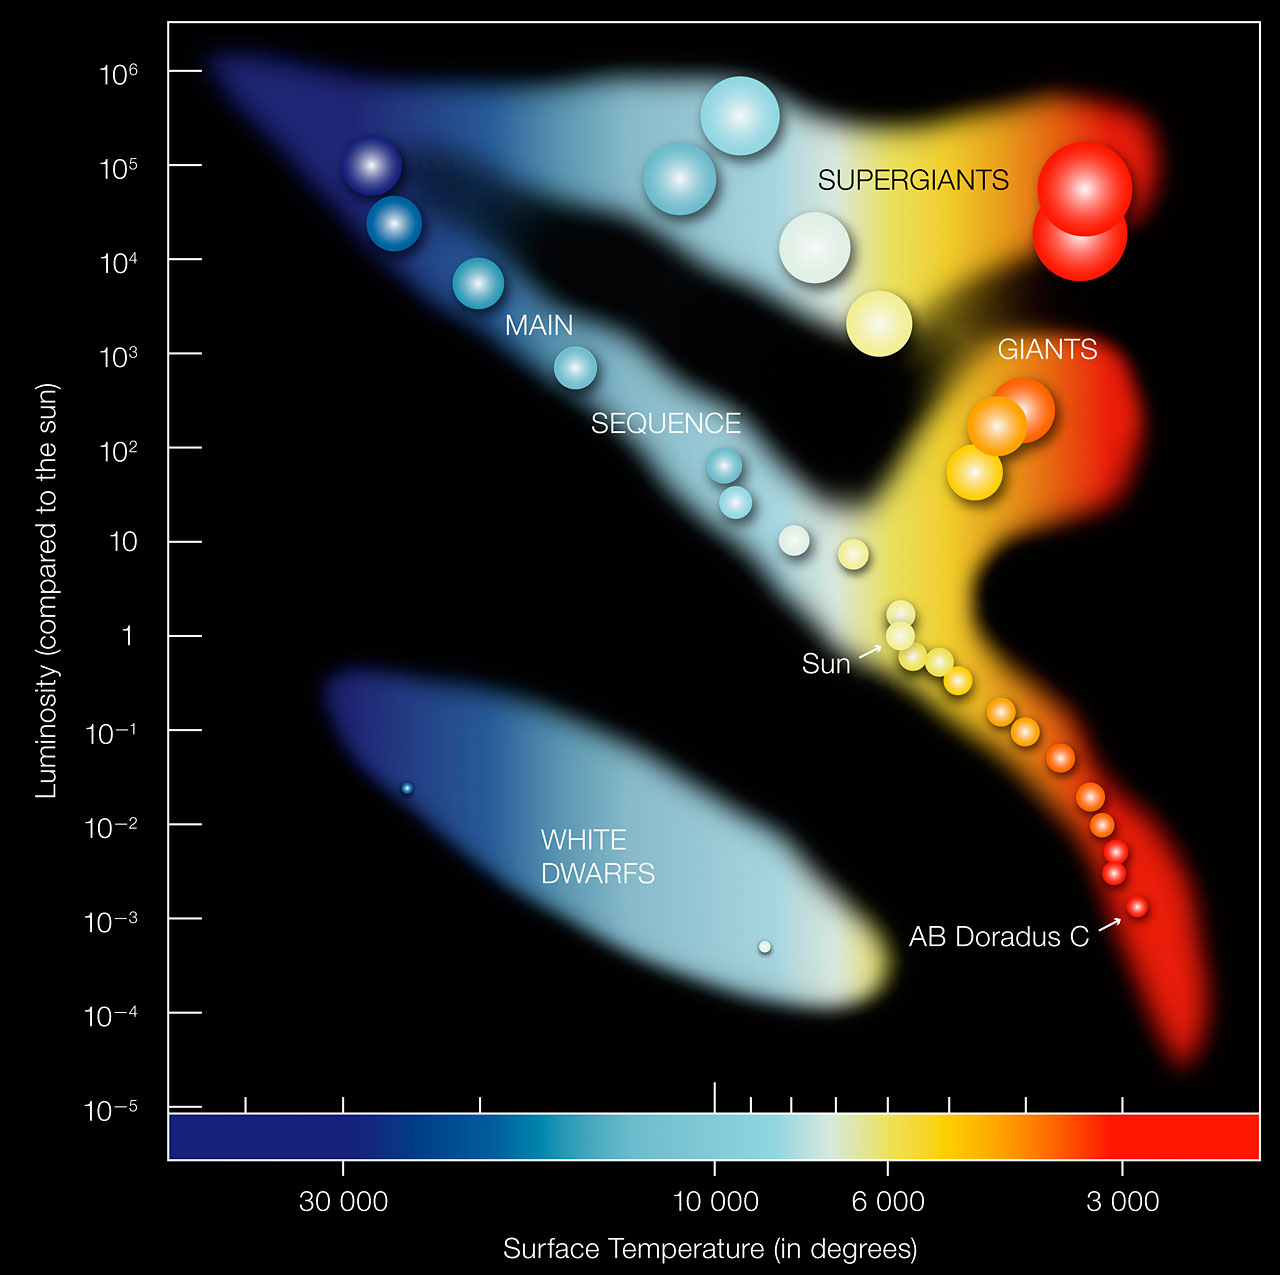
\includegraphics[width=\textwidth]{img/hz-diagram-eso0728c}%
  		\caption{\textbf{Herztsprung-Russell Diagram}: 
  		In the Hertzprung-Russell diagram the temperatures of stars are plotted against their luminosities. The position of a star in the diagram provides information about its present stage and its mass. Stars that burn hydrogen into helium lie on the diagonal main sequence. The Sun is situated about the middle of the main sequence. \textbf{Credit}:ESO}
  		\label{fig:hr-diagram}
\end{figure}

The relation between the stellar properites of luminosity, effective temperature (or spectral type) and radius were studied by the physicists Ejnar Herztsprung and Henry Russell at the beginning of the 20\textsuperscript{th} century. Their studies produced a very important aid in studies of stellar evolution, the Hertzsprung-Russell Diagram, or simply HR diagram (Figure\ref{fig:hr-diagram}). One might have expected a uniform distribution of temperatures and luminosities, but it is found that most stars lie on the Main Sequence -- the diagonal going from upper left to lower right. On the other diagonal, from lower left to upper right, the radii of the star increase (in accordance to equation \ref{eq:essential-relation}. It is notable as well that the yellow and red stars (spectral types G–K–M) appear to be clustered into either the dwarf stars of the main
sequence or the giants. The supergiants have an almost horizontal sequence, while the red giant branch rises from the main sequence around the temperature mark of the Sun. Below the main sequence, there is the group of white dwarfs, which are quite fainth and difficult to observe.

Protostars enter the main sequence as their radius decreases and their temperature increases. In the main sequence stars are most stable, but they will eventually exhaust all the hydrogen. When this happens, the star leaves the main sequence and, depending on thier mass, they have various destinies. Low mass stars ($\sim 0.5 \rm{M_\odot}$) will not have sufficient gravity to heat the core to high enough temperatures and pressures for fusing helium. They will cool down and become Red Dwarfs, like \textit{AB Doradus C} in Figure \ref{fig:hr-diagram}. \textit{AB Dor C} has a temperature of about $3 000 \rm{K}$ and a luminosity which is $0.2\%$ that of the Sun and it will never leave the main sequence. Stars similar to the Sun will expand and shed their exterior layers, as they run out of hydrogen, they will then collapse again before burning their Helium reserves and become a Red Giant before collapsing again into a White Dwarf. Bigger stars will expand to Super Giants, fusing more heavy elements. They will end their lives most spectacularly with a supernova, which will leave behind a neutron star for a star with more than $1.4 \rm{M_\odot}$ or a black hole for stars with a mass of more than $3 \rm{M_\odot}$ \citep{Reese2005}.


\subsection{Variable Stars}
\label{variable-stars}

Stars with changing brightness (or absolute magnitudes) are called \textit{variables} or \textit{variable stars} (about 40,000 stars known or suspected to be variable \citep{Karttunen2017}). Technically, all stars are variable, given that their structure and brightness change as they evolve. Although the changes are usually slow, some evolutionary phases can be extremly rapid, or may present periodic variations, for example pulsations of the outer layers of a star. Small variations in stellar brightness are also caused by dark or light spots on a star's surface, as it rotates about its axis. The magnitude variation as a function of time is called the lightcurve of a star (Figure \ref{fig:lightcurve}). From this the amplitude and period of the variation can be determied, if periodic. 

\begin{figure}[hbt!]
		\centering
		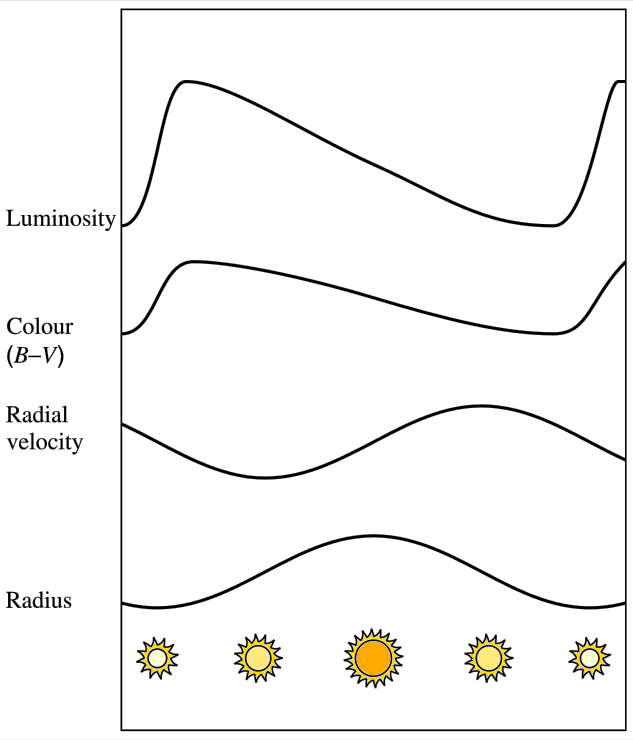
\includegraphics[width=0.4\textwidth]{img/lightcurve-v2}%
  		\caption{Variation of brightness, color and size of a cepheid \protect\footnotemark[1] during its pulsation. The uppermost curve, describing luminosity is called the lightcurve. \textbf{Credit}: Adapted from \citep{Karttunen2017}}
  		\label{fig:lightcurve}
\end{figure}

Variables are classified based on the shape of their lightcurve, the spectral class and the observed motions in mainly three categories: pulsating, eruptive and eclipsing variables. A pulsating variable is an intrinsic variable, whose exterior layers are dillating and contracting, trying to reach an equilibrium between the gravitational force pushing inwards and the gas pressure pushing outwards. In the case of many pulsating variables (including cepheids\footnote{Among the most important pulsating variables are the \textbf{cepheids}, named after $\delta$ \textit{Cephei}. They are supergiants of spectral class F–K, with periods of 1-50 days and amplitudes of 0.1–2.5 magnitudes in their variability}) the period of variation of the star is proportional to its luminosity. The diameter may double during the pulsation, but usually the main cause of light variation is the periodic variation of surface temperature. As seen in equation (\ref{eq:essential-relation}) $L \propto T_e^4$ and a small change in effective temperature leads to a large brightness variation. Stars with surface temperatures of 6000–9000 K are liable to this instability and the corresponding section of the HR diagram is called the cepheid instability strip. There are various pulsating variable stars with periods up to 500 days. 

The eruptive variables exhibit instead of a regular pulsation a sudden outburst in which material is ejected into space. These star are usually surrounded by a gas shell or interstellar matter. Flare stars are young stars wich present flare outbursts on the surface at irregular intervals. Such a flare can cause a brightening by up to 4-5 magnitudes \citep{Karttunen2017}.  Although this process is still not fully understood, it is common that a protostar and its accretion disc to cause jet-like flares as seen in Figure \ref{fig:flare}.

\begin{figure}[hbt!]
		\centering
		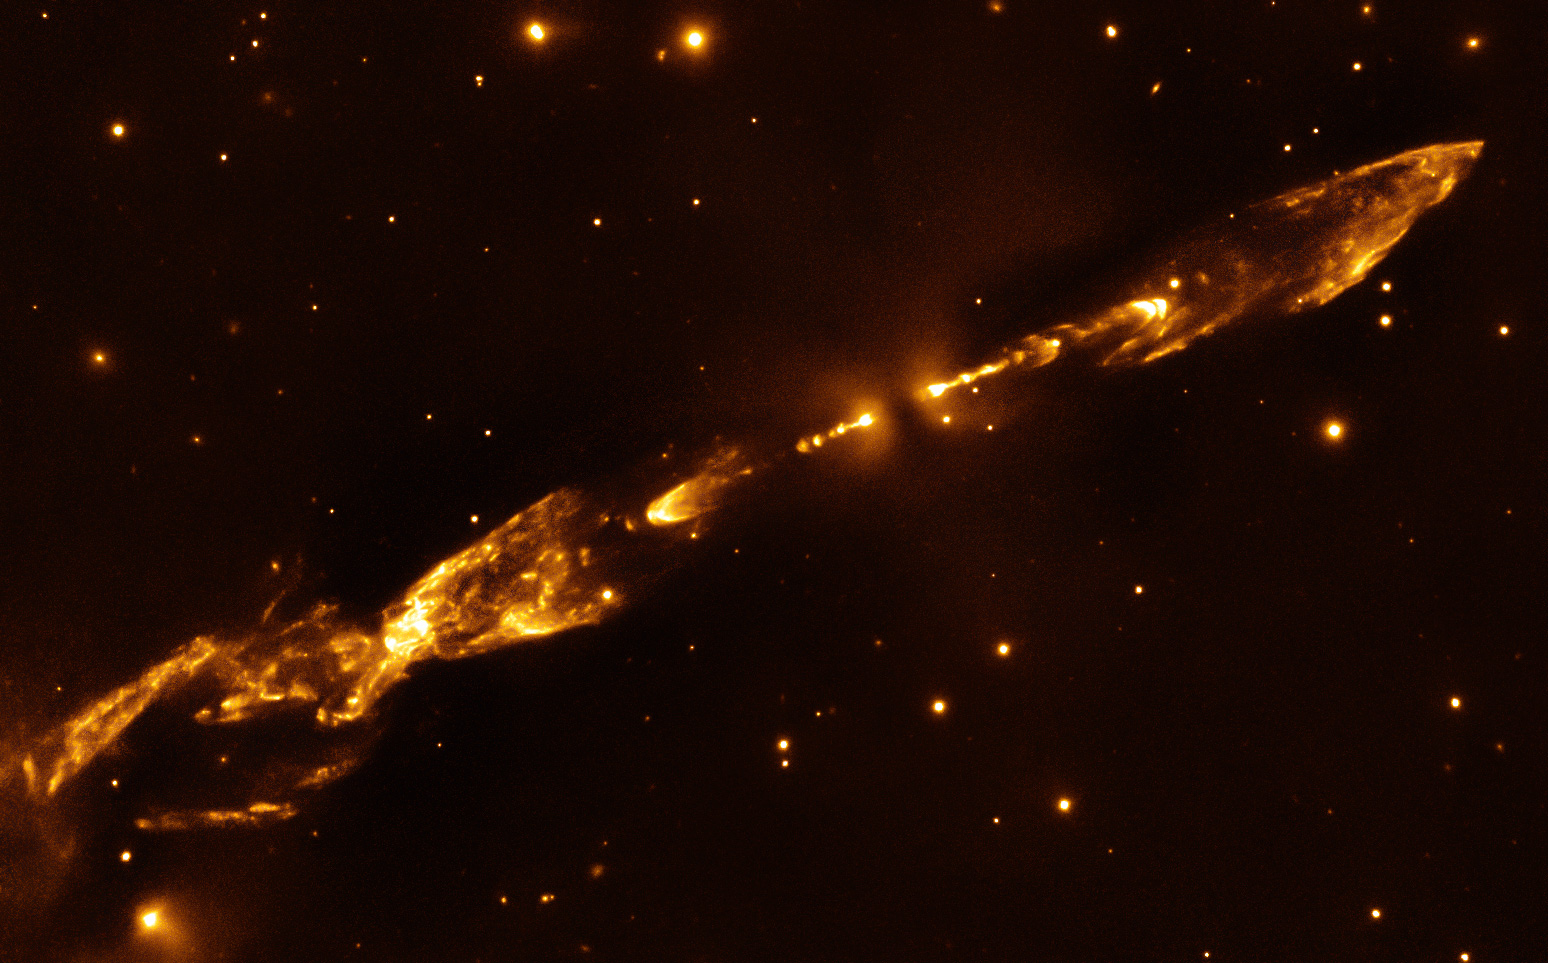
\includegraphics[width=\textwidth]{img/flares-potw1541a}%
  		\caption{Image of Herbig-Haro object (HH) 212, located in a dense star-forming region of the Horsehead Nebula with very large almost symmetric flares in orange. The central star is very young (thousands of years old) and it can be observed masked by the surrounding dusty disk (central dark region from which flares seem to originate), which is seen here edge-on. The star's pulses vary quite regularly, and over a short timescale (maybe even as short as 30 years). Further out from the centre, large bow shocks caused by ejected gas colliding with dust and gas at speeds of several hundred kilometres per second spread out into interstellar space. \textbf{Credit}: ESO/M. McCaughrean \url{https://www.eso.org/public/images/potw1541a/}}
  		\label{fig:flare}
\end{figure}

A flare lights up in a few seconds, and fades away in a few minutes, but the same star can flare up several times in one day. Novae and supernovae are also included in this category, but the T Tauri are the most interesting flare stars, and are one of the topics of concern of the present thesis. These stars are newly formed and just contracting toward the main-sequence. Such stars, in the process of formation, may change brightness very rapidly and commonly have irregular brightness variations (\textit{FU Orionis} brightened in 1937 by 6 magnitudes). In 1969 \textit{V1057 Cygni} brightned by six magnitues, and had remained fairly constant since.

The third category is the eclipsing variables. As the name suggests, these are usually binary systems in which the components periodically pass in front of each other. The variability is not related to any physical change in the star, and is apparent. 
In addition, a few rotating varaibles with an uneven distribution of temperature on the surface are known. They have periods of about 1 to 25 days and the changes are small, less than 0.1 magnitudes.

\subsection{T Tauri stars}

T Tauri stars were briefly mentioned in the previous section \ref{variable-stars}. It is important to define them, as they are the type of stars of interest to this thesis, and the relevant basis has been explored in order to fully understand their definition. They are a type of young pre-main-sequence variable stars in the process of contracting towards the main sequence. T Tauri stars usually have masses lower than 2 solar masses, and are of spectral types F, G, K or M. Their surface temperatures are similar to those of main-sequence stars of the same mass, but they are significantly more luminous because their radii are larger. Similar young pre-main-sequence stars, are Herbig Ae/Be type stars. They have masses between 2 and 8 $M_{\odot}$ and are of spectral type A or B. They may sometimes show significan brightness variability. As they are in not in the main sequence yet, both stellar types are not burning hydrogen, and are powered by gravitational energy released as the stars contract.


\section{Circumstellar Disks}

\begin{figure}[hbt!]
		\centering
		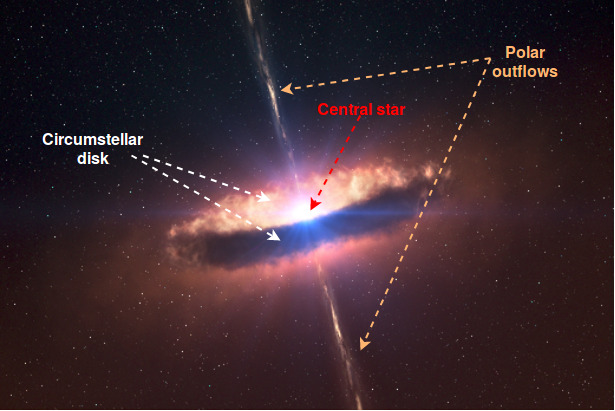
\includegraphics[width=\textwidth]{img/circumstellar-disk-eso1029a}%
  		\caption{Artist impression (with added annotations) of pre-main-sequence star with disk. The disk extends to about 130 AU, and has a mass similar to the star. Jets can be observed at either pole of the star, spewing matter. \textbf{Credit}: ESO/L. Calçada/M. Kornmesser \url{https://www.eso.org/public/images/eso1029a/}}
  		\label{fig:schema}
\end{figure}

As seen in section \ref{star-formation}, as clouds collapse into protostars, much of the the angular momentum of the collapsing
cloud is taken up by a circumstellar disk of gas and dust, which lasts 1–10 Myr before being photodissipated. It is thought that angular momentum has been significantly reduced by magnetic coupling between the star and the disk and also through the outflow in the poles, which is strongest during the protostellar phase. A schematic of a typical circularly-symmetriccal disk can be seen in Figure \ref{fig:schema}. Even though the disks usually contain only a few percent of the material going into a young star, they are of great interest to study, because they are the place where planets may form.

How common are circumstellar disks? Using data from the IRAS sky survey, two teams \citep{Cohen1989} and \citep{Strom1989} discovered that approximately half of the T-Tauri stars observed have far infrared spectral energy distributions (SEDs), characteristic of heated dust and not of the photosphere. The relative low visual exctinction (absobed light from the star) suggested that the dust was in a flattened distribution. The first pictures of disks taken with the Hubble Space Telescope demonstrated clearly that the dust distribution followed the thoretical pattern of a disk \citep{Bechwith1999}. Circumstellar disks (\ref{fig:disk-artist-impression}) are gently flared in the outer region due to the warming of the matter, and have some edge at a distance from the star (called further inner radius of the disk $R_{in}$ in as in Figure \ref{fig:flare}), and are heated mainly by radiation (as opposed to accretion). Most young disks are also accompanied by mass losses in columns around the polar axes.%
\vspace*{-35mm}
\begin{figure}[h!]
	\begin{subfigure}[t]{0.9\textwidth}
	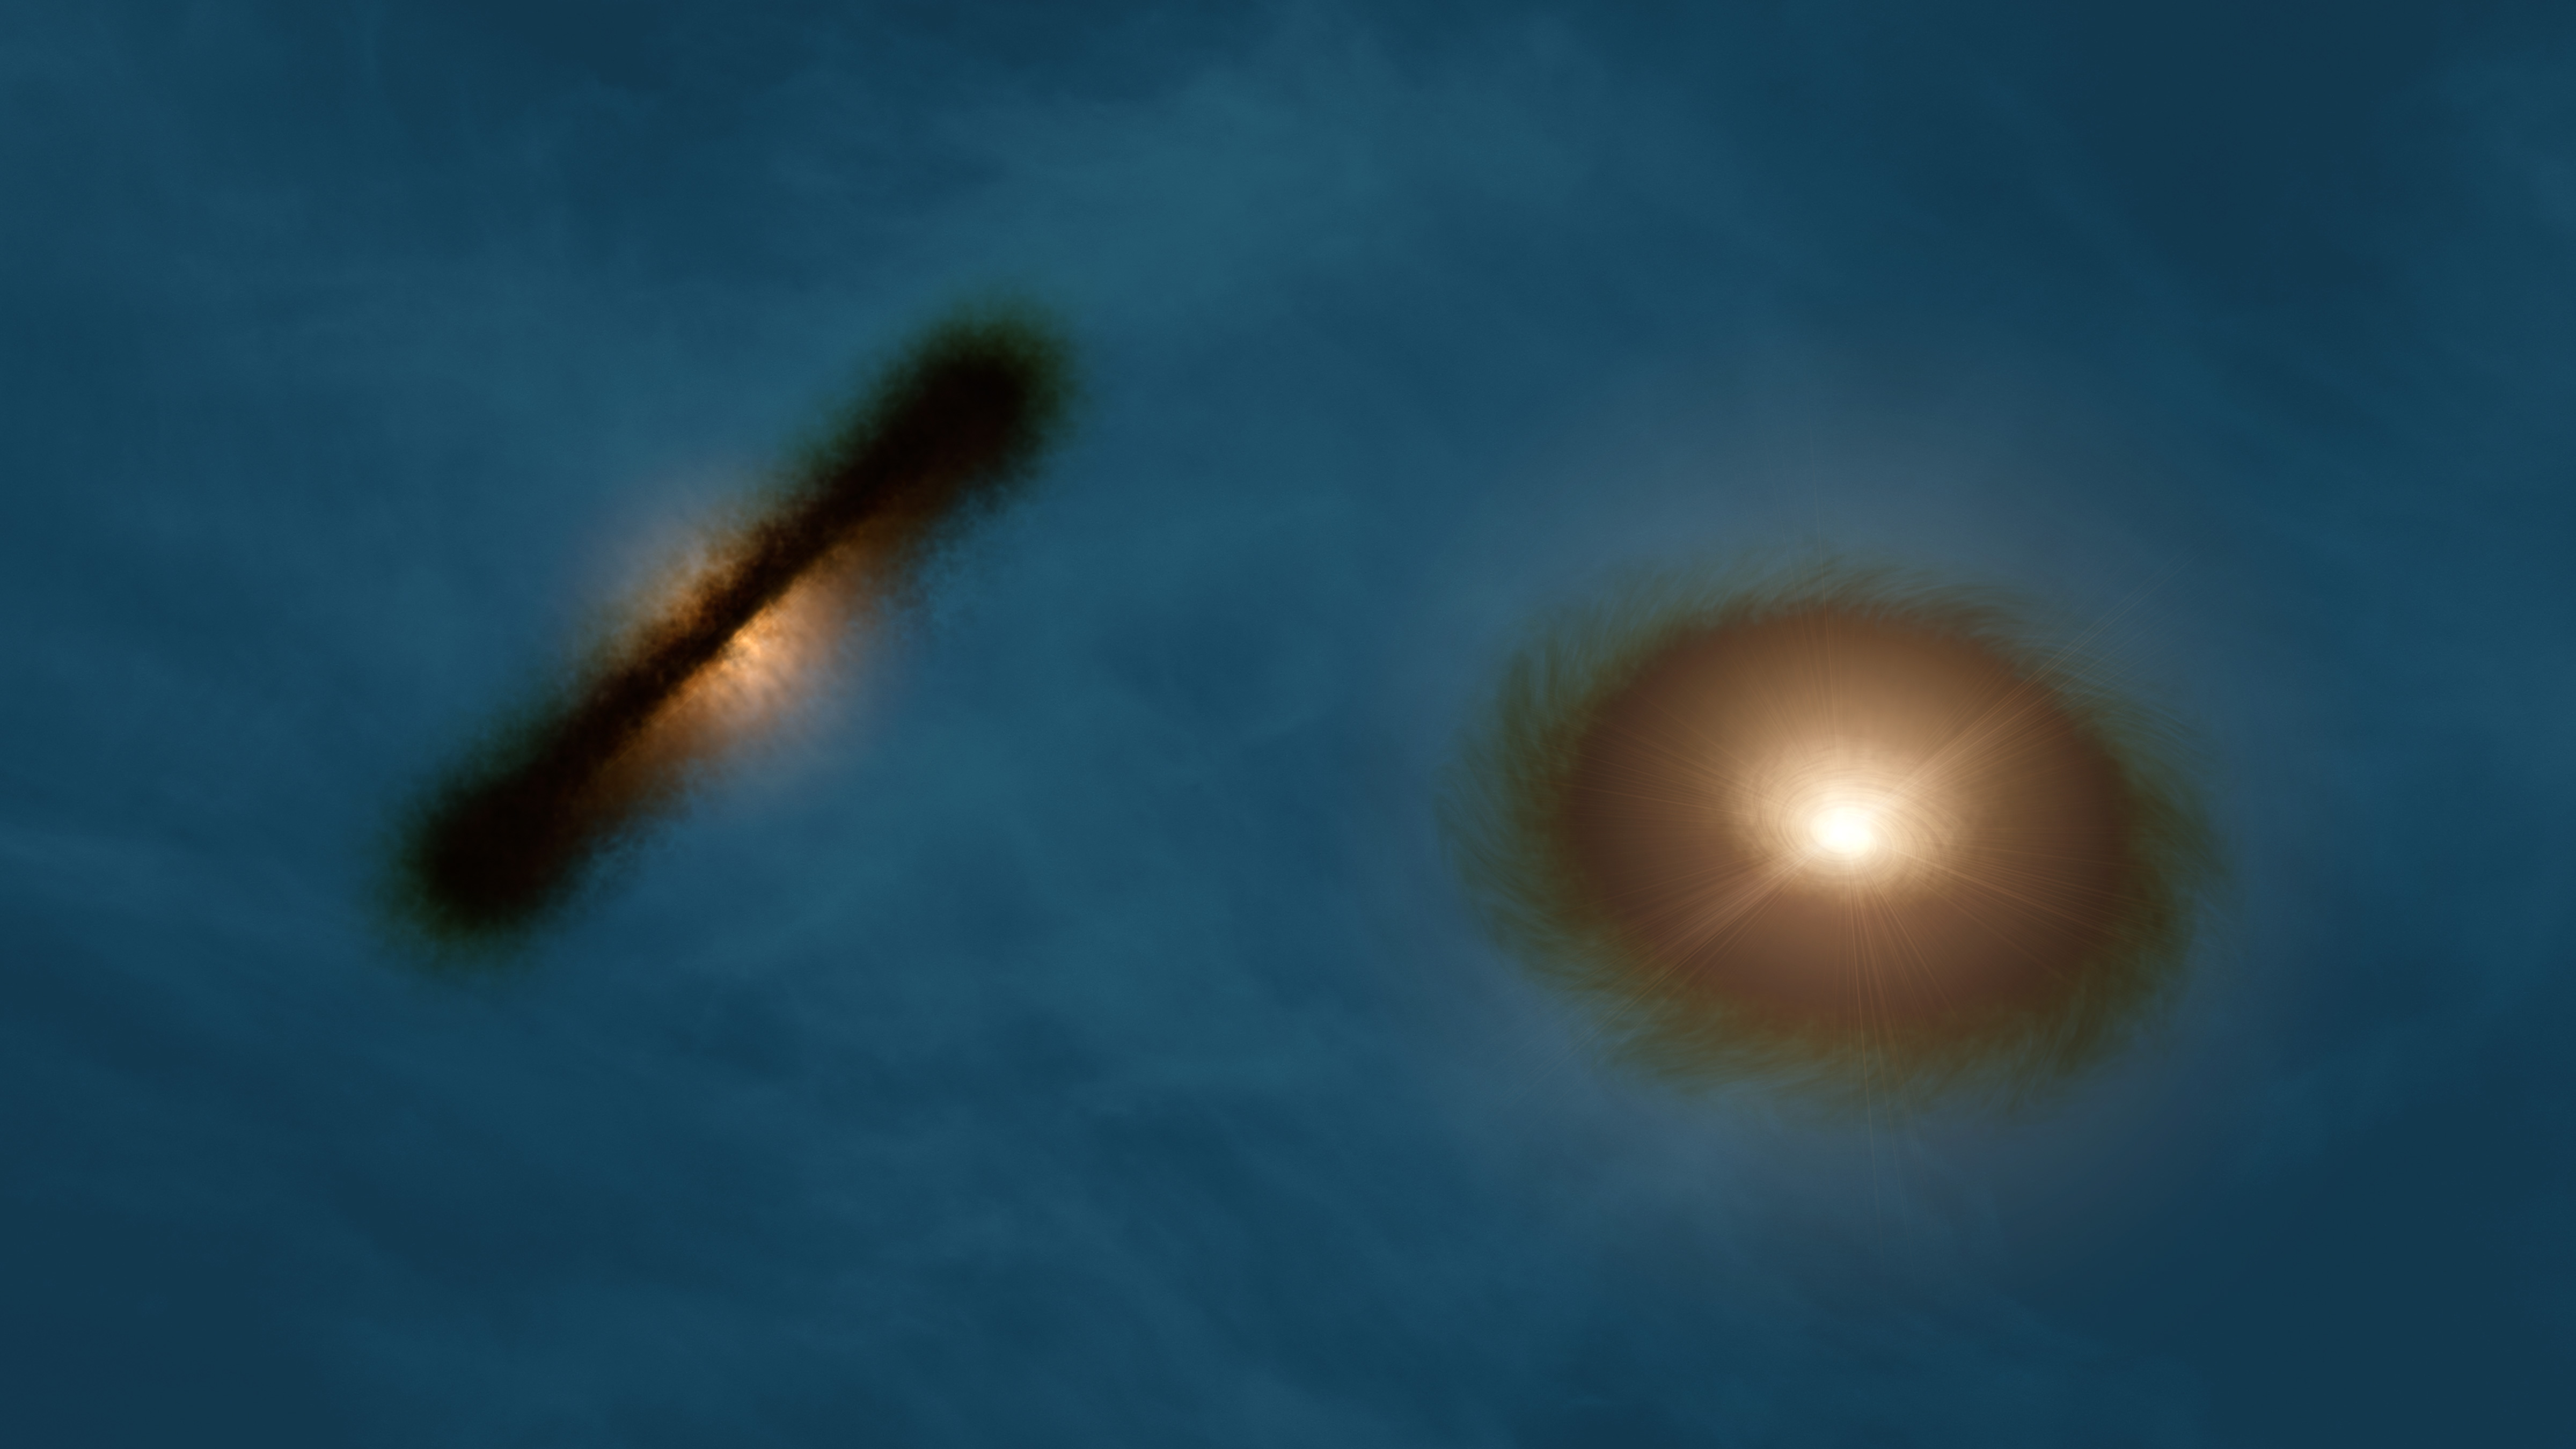
\includegraphics[width=\textwidth]{img/circumstellar-disk-eso1423a}
	\caption{Artist impression of two circumstellar disks. The one on the left is seen edge on by the observer, while the disk on the right is almost face-on with a slight incline towards the observer. }
	\label{fig:disk-artist-impression}
	\end{subfigure}\par\bigskip
	\begin{subfigure}[t]{0.9\textwidth}
	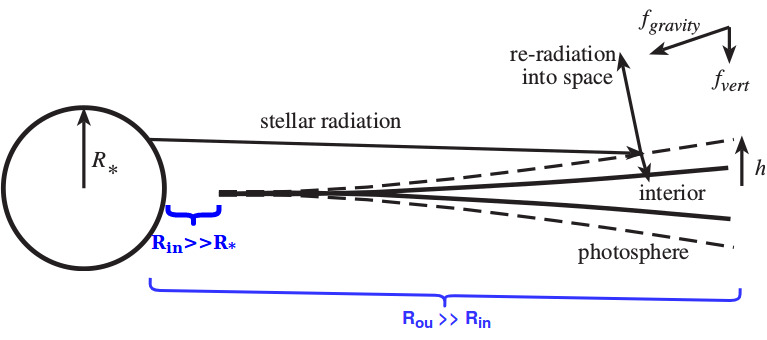
\includegraphics[width=\textwidth]{img/flare}
	\caption{Schematic of star with section through flared circumstellar disk. The radius of the star $R_{*}$ is usually a few solar radii $R_{\odot}$, while the rim of the disk approaches the star usually at a couple of astromical units. Between the star and the inner radius of the disk $R_{in}$ all dust is considered to have been accreted, due to unstable orbits, or the temperatures are too high for the dust to exist, making the dust density in this area nul. The disks outer radius is hard to distinguish as a low density, but non-zero distribution of dust may exist beyond the outer radius $R_{out}$, which is usually a couple of hundred astronomical units.}
	\label{fig:flare}
	\end{subfigure}
\end{figure}

\newpage
\subsection{Interstellar Dust}

Though originally thought as transparent, the interstellar medium is actually filled with dust, which also forms circumstellar disks. The dust was first observed when deducing that the apparent magnitude of stars is dimmed by some intervening material. Extinction due to dust varies with direction and is due to the particles having diameters near the wavelength of light ($0.01 - 0.2 \mu m$. Such particles scatter light extremly efficiently. Gas can also cause extinction by scattering, but the efficiency per unit mass is much smaller. 

Interstellar dust particles can cause extinction in two ways \citep{Karttunen2017}
\begin{itemize}
\item Through absorption the radiant energy is transformed into heat, which is then re-radiated at infrared wavelengths corresponding to the temperature of the dust particles.
\item Through scattering the direction of light propagation is changed, leading to a reduced intensity in the original direction of propagation.
\end{itemize}

For simplicity in calculating the coefficient of extinction $C_{\rm{ext}}$ for dust particles, they are assumed to be spheres with the same radius $a$, and therefore geometrical cross-section $\pi a^2$.

\begin{equation}\label{eq:coeff-ext}
	C_{\rm{ext}} = Q_{\rm{ext}} \pi a^2,
\end{equation}
%
where $Q_{\rm{ext}}$ is the extinction efficiency factor. Consider a volume element with cross section $dA$, incident to the radiation, and length $dl$. If the particle density is $n$, the total number of particles in a unit volume is $N= n dA dl$, while the fraction of the area covered by the particles will be $C_{\rm{ext}}/dA$. On the basis of the previous equation (\ref{eq:optical-depth}), the optical depth over a path of length $r$ can be expressed as a function of the extinction coefficient as: 

\begin{equation}
	\tau = N \sigma = \int_0^r n C_{\rm{ext}} dl \approx C_{\rm{ext}} \overline{n} r \approx Q_{\rm{ext}} \pi a^2 \overline{n} r
\end{equation}
%
where $\overline{n}$ is the average density along the path.

The extinction factor $Q_{\rm{ext}} = Q_{\rm{abs}} + Q_{\rm{sca}}$ is the sum of the absorption and the scattering extinction factors, and can be calculated for a given frequency from the quantity $x = 2 \pi a/ \lambda$, where $a$ is the radius of the dust particles, and the refractive index $m$ ($Q_{\rm{ext}} = Q_{\rm{ext}}(x, m)$). When $x << 1$, the particle is much smaller than the wavelength and elastic or Rayleigh scattering occurs, whereas for $x \geq 1$ Mie scattering occurs. An observable phenomena that occurs due to dust is the \textbf{\textit{reddening}} of stars due to the fact that extinstion becomes larger for shorter wavelengths. This means that going from red to ultraviolet the extinction is roughly inversely proportional to wavelength. For this reason, the light of distant stars is redder than would be expected on the basis of their spectral class. At the same time, if a dust cloud is close to a bright star, it will reflect much of the light, moreso in the blue end of the spectrum. Indiviudual dust clouds can be observed as bright reflection nebulae. 

\begin{figure}[ht]
	\begin{subfigure}[t]{0.45\textwidth}
		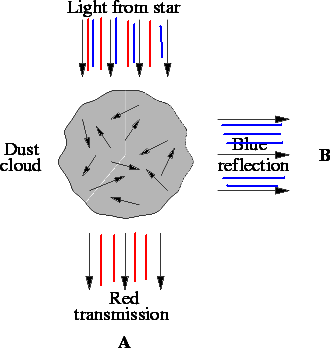
\includegraphics[height=5cm]{img/dust1}
		\subcaption{}
		\label{fig:dust1}
	\end{subfigure}\hfill%
	\begin{subfigure}[t]{0.45\textwidth}
		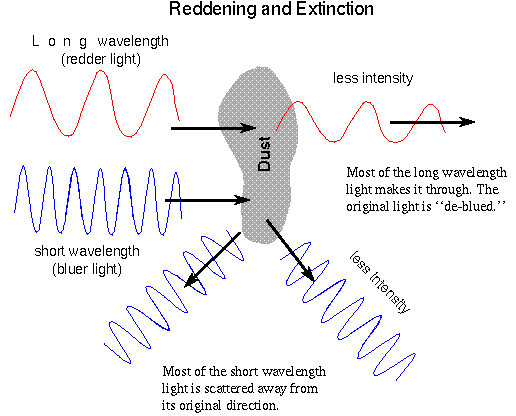
\includegraphics[height=5cm]{img/dust2}
		\subcaption{}
		\label{fig:dust2}
	\end{subfigure}%
\caption{Dust extinction and scattering}
\label{fig:barnard68}
\end{figure}

Dust particles polarize light from the stars. Since this effect could not be produced by spherical particles, the interstellar dust particles must be non-spherical in shape. Through alignment by the interstellar magnetic field, dust particles will polarize radiation passing through a cloud. The degree of polarisation and its wavelength dependence rest on the properties of the dust particles. In addition to scattering radiation, dust also absorbs energy and re-radiate it at infrared wavelengths, corresponding to their temperature. For interstellar dust (including in dark nebulae) at $10 - 20 \rm{K}$, the corresponding peak accourding to Plack's law would be at $300 - 150 \rm{\mu m}$, while for dust at the inner edge of a circumstellar disk, near a hot star, the temperatures may be $100 - 600 \rm{K}$ and the maximum emission is then at $30 - 5 \rm{\mu m}$, illustrated in Figure \ref{fig:dust-planck}. Dust can be detected and observed in the infrared due to it's strong thermal emission. 
	
\begin{figure}[ht]
	\begin{subfigure}[t]{0.45\textwidth}
		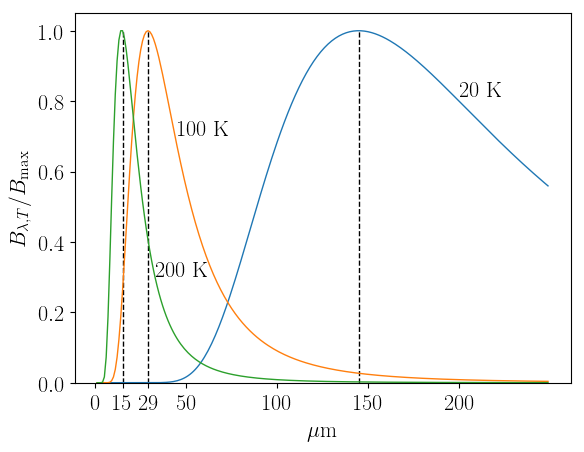
\includegraphics[height=5cm]{img/planck}
		\subcaption{}
		\label{fig:dust-planck}
	\end{subfigure}\hfill%
	\begin{subfigure}[t]{0.45\textwidth}
		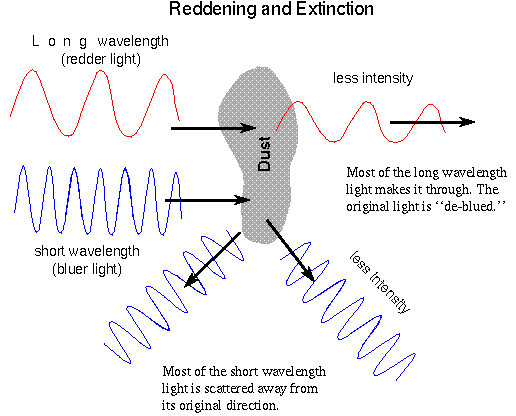
\includegraphics[height=5cm]{img/dust2}
		\subcaption{}
		\label{fig:dust2}
	\end{subfigure}%
\caption{Dust extinction and scattering}
\label{fig:barnard68}
\end{figure}

From the peaks in the extinction curves, it may be concluded that interstellar dust contains water ice and silicates, as well as graphite. A typical composition \citep{Weingartner2001} is 63.5\% astrosilicate combined with carbon in different polarisations. The sizes of the grains, deduced from their scattering properties are usually smaller than $1 \rm{\mu m}$. Dust grains are assumed to be formed in the atmospheres of stars of late spectral types (K, M), as gas condenses into grains, which are then expelled into interstellar space by radiation pressure. Although the mass of interstellar gas is a hundred times larger than that of dust, gas is less easily observablea as it does not in general cause great extinction of light. 
